% Semantiek en Correctheid werkstuk over transacties
%
% 2009
\documentclass[twoside,fleqn]{artikel3}

\title{Transacties in While}
\author{Mehdi Aqadjani Memar, Joost Kraaijeveld, Louis Onrust}

\usepackage{amsmath}
\usepackage{semantic} % Voor documentatie kijk hier: http://tug.ctan.org/tex-archive/macros/latex/contrib/semantic/
\usepackage[dutch]{babel}
\usepackage{hyperref}
\usepackage{tikz}
\usetikzlibrary{arrows,shadows,decorations.pathmorphing,shapes}
\usepackage{listings}
\usepackage{multicol}
\usepackage{longtable}
\usepackage{multirow}
\usepackage{dsfont}
\usepackage{color}
\usepackage{ifthen}
\usepackage[hmargin=2.5cm,vmargin=3.5cm]{geometry}
\usepackage{byname}
\usepackage{marginnote}
\usepackage{boxedminipage}
\usepackage{makeidx}
\usepackage{underscore}
\usepackage{fancyhdr}
\pagestyle{fancy}
\fancyfoot{} % clear all footer fields
\fancyfoot[LE,RO]{\thepage}


\bibliographystyle{apalike}

\newenvironment{functie}[1]{
\begin{boxedminipage}[t]{\textwidth}
\vspace{-.25em}\textbf{#1}\vspace{.25em}
}{\end{boxedminipage}}

\newcommand\functielabel[1]{\textit{#1}}
\newcommand\inlinecomment[1]{{\color{red}#1}}
\newcommand\syncat[1]{\textbf{#1}}
\newcommand\functienaam[1]{\kw{#1}}
\newcommand\functiebody[1]{\newline $\rightarrow$ \textsl{#1} }
\newcommand\functievariabele[1]{\text#1}
\newcommand\functieargument[1]{\newline $\rightarrow$ \textsl{#1} }
\newcommand\functieresultaat[1]{\newline $\leftarrow$ \textsl{#1} }
\newcommand\functieopmerking{\newline{}\newline\(\textrm{\underline{Opmerking}}\): }
\newcommand\functieomschrijving{\newline\strut\newline}
\newcommand\osstep[3]{\ensuremath{\langle#2\rangle
						=>\ifthenelse{\equal{#1}{def}}{}{_{#1}}
						\ifthenelse{\equal{#3}{s}}
							{s}
							{ %else
							\ifthenelse{\equal{#3}{s'}}
								{s'}
								{ %else
								\langle#3\rangle
								}
							}}
						} % type lhs rhs
\newcommand\kw[1]{\textnormal{\texttt{#1}}} % keyword
\newcommand\var[1]{\textnormal{\textsl{#1}}} % variable
\newcommand\Index[2][def]{#2\ifthenelse{\equal{#1}{def}}{\index{#2}}{\index{#1}}}
\newcommand\Section[2][def]{\section{#2}\ifthenelse{\equal{#1}{def}}{\label{sec:#2}}{\label{sec:#1}}}
\newcommand\Subsection[2][def]{\subsection{#2}\ifthenelse{\equal{#1}{def}}{\label{ssec:#2}}{\label{ssec:#1}}}
\newcommand\Subsubsection[2][def]{\subsubsection{#2}\ifthenelse{\equal{#1}{def}}{\label{sssec:#2}}{\label{sssec:#1}}}
\renewcommand\emph[1]{\textbf{#1}}
\renewcommand\lstlistingname{Functie}
\renewcommand\thepart{\Alph{part}}
\renewcommand\thesection{\thepart\ \arabic{section}}

\lstdefinelanguage{trans}{
	morekeywords={
		func,is,spawn,wait,var,
		if,then,else,
		true,false,undef,
		start,end,set\_result,
		start\_transaction,collect\_votes,
		commit\_transaction,rollback\_transaction
	},
	otherkeywords={
		=, :=, ::=, <, +, ;
	},
	sensitive=false,
	literate={ epsilon }{{$\epsilon$}}1 ,
}
\lstset{
	basicstyle=\small,
	keywordstyle=\bfseries,
	tabsize=2,
	language={trans},
}

\let\itemOld\item % boldface math in \item's too
\makeatletter
\@addtoreset{section}{part}
\renewcommand\item[1][]{%
	\def\@tempa{#1}
	\ifx\@tempa\@empty\itemOld\else\boldmath\itemOld[#1]\unboldmath\fi%
}
\def\maketitle{\Huge\@title\vspace{.35em}\newline\normalfont\Large\@author\normalsize}
\makeatother

\newcommand\markers[1]{%
\marginnote{%
\vspace{-2cm}%
\begin{tikzpicture}[remember picture,yshift=1cm]%
\pgfsetbaseline{40pt}
\draw (0,1) node[] (inNode) {\hspace{-2.5cm}#1};%
\draw (-1.5,1) -- (-2.5,1);%
\end{tikzpicture}%
}%
}%

\newlength{\sLength}
\settowidth{\sLength}{$s$}
\newlength{\maxFunctionLength}
\settowidth{\maxFunctionLength}{\texttt{end\_rollback}}

\newcommand\marker[1]{%
\marginnote{%
\vspace{-2cm}%
\begin{tikzpicture}[remember picture,yshift=1cm]%
\pgfsetbaseline{40pt}
\draw (0,1) node[] (inNode) {\hspace{2.5cm}#1};%
\draw (1.5,1) -- (2.5,1);%
\end{tikzpicture}%
}%
}%

\newcounter{threadnum}
\global\def\upperhalfbar{0.125}
\global\def\lowerhalfbar{-\upperhalfbar}
\global\def\twidth{\textwidth-0.4pt}
\setlength{\unitlength}{1cm}
\tikzstyle{inststyle}=[rectangle, draw, anchor=west, minimum
height=0.8cm, minimum width=1.6cm, fill=white,
drop shadow={opacity=1,fill=black}]
\tikzstyle{marker}=[anchor=base]

\makeindex

% Elk hoofdstuk krijgt een eigen \input.
\begin{document}

\begin{titlepage}
\maketitle
\vfill
\begin{multicols}{2}
\tableofcontents
\end{multicols}
\newpage
\strut
\thispagestyle{empty}
\end{titlepage}
\section*{Inleiding}

Een While programma zoals beschreven in het boek \cite{SemanticsWithApplications} is in
essentie een lineair uitvoerbare sequentie van atomaire statements.

In dit stuk wordt een uitbreiding van While beschreven waarbij arbitraire verzamelingen van statements kunnen worden
gebundeld tot atomaire eenheden (transacties) die bovendien parallel aan elkaar kunnen worden uitgevoerd
(parallellisme).

Beide concepten kunnen individueel gebruikt worden binnen een programma; interessant wordt het pas wanneer er gekeken
wordt naar de mogelijkheden die een combinatie van transacties en parallellisme samen teweeg kunnen brengen.

De opbouw van het werk wordt opgedeeld in drie verschillende stukken:
\begin{enumerate}
  \item In het eerste stuk worden de uitbreidingen behandeld die nodig zijn
  \item In het tweede stuk wordt de formalisatie besproken van de uitbreidingen
  \item In het laatste stuk wordt vervolgens een programma besproken en de
  scenario's die voor kunnen komen worden besproken aan de hand van bewijzen in de vorm van afleidingen
\end{enumerate}


\part{Uitbreidingen}
In het werk zal voortdurend gebruik gemaakt worden van het begrip programma. Een programma in essentie niets anders dan
een verzameling van functies (zie~\ref{sec:Functies}). Deze functies zijn op hun beurt weer een sequentie van
statements.

Een programma in While is ook een serie statements, maar hier worden verder geen eisen aan gesteld;
\(\mathcal{S}|[z:=x|](x\mapsto5)\) kan ook al een geldig programma zijn. Bij ons is een programma hetgeen de programmeur
opschrijft (zie~\ref{sec:Programma}). Dus programma als begrip omvat alles wat minimaal ge\"eist wordt door de
specificaties, en dit omvat ook het begrip programma uit While, de sequentie van statements. In deze programma's mag
gebruik gemaakt worden van alle mogelijkheden die While biedt, maar nu zijn er ook een aantal uitbreidingen die gebruikt
mogen worden zoals het opstarten van parallelle taken en het opstarten van een transactionele omgeving met alle voor- en
nadelen die ermee verbonden zijn.

\Section{Executieomgeving}

Een programma staat meestal niet op zich. In de meeste gevallen wordt een programma opgestart binnen een
besturingssysteem. Een dergelijke omgeving zorgt ervoor dat allerlei infrastructuur niet door ieder programma zelf
ge\"implementeerd hoeft te worden. In een aantal gevallen zullen we omwille van abstractie gebruik maken van een
dergelijke omgeving, hier \Index{executieomgeving} genoemd.

Het is de taak van de executieomgeving om het programma op te starten en alle benodigde variabelen te initialiseren.
Verder zorgt de executieomgeving voor het beheer van de taken en zorgt ervoor dat communicatie tussen de taken mogelijk
is.

\Subsection{Globaliteit}
De executieomgeving is de meest globale omgeving. Dat wilt zeggen dat de executieomgeving alles kan overzien wat er
gebeurt in het programma; het heeft dus zicht op alle taken, variabelen en de algemene progressie.

Omdat onze taal het niet toestaat dat een taak variabelen aanspreekt of wijzigt buiten de omgeving van de taak, levert
dit in gevallen wanneer de ene taak bijvoorbeeld een resultaat terug wilt geven aan een andere taak, problemen op. Om
dit toch goed te laten verlopen wordt er voor de interactie tussen de twee taken gebruik gemaakt van de
executieomgeving als tussenpersoon, zodat de overdracht van gegevens niet alleen goed verloopt, zonder de regels te
overtreden, maar ook om deze overdracht als atomaire stap te beschouwen.

Een andere belangrijke taak van de executieomgeving is het in de gaten houden van de taken. Zeker in het geval van
interactie tussen taken (zoals die in transacties bijvoorbeeld plaats zullen gaan vinden) is het erg handig om te weten
of de taak met wie je wilt samenwerken \"uberhaupt nog wel bestaat. De executieomgeving zal niet per se publiekelijk
maken dat een taak gestorven is, maar wanneer er naar gevraagd wordt kan er onder alle omstandigheden een antwoord
verkregen worden betreffende de status van de taak.

In sommige gevallen maakt de executieomgeving ook bepaalde dingen publiekelijk, dit geldt voor de zogenaamde labels. Op
elk moment is voor elke taak bekend welke functies er allemaal bestaan, maar ook welke andere taken er zijn en welke
transacties er allemaal bezig zijn. Labels die expliciet lokaal zijn binnen de taak zijn de variabelen, dit onder
andere om te verzekeren dat data-integriteit gegarandeerd kan worden (met als uitzondering de executieomgeving, die deze
variabelen wel kan inzien).

Het is voor de individuele taken binnen een programma niet mogelijk om onderling direct te communiceren. Eventuele
communicatie (zoals het wachten op elkaar en het doorgeven van resultaten etc) gebeurt door dit aan de executieomgeving
``te vragen'' door middel van functieaanroepen/systemcalls. Alle communicatie tussen de executieomgeving en individuele
taken gebeurt atomair: er is nooit sprake van enig raceconditie als gevolg van deze communicatie.

De state van de executieomgeving is vergelijkbaar met een environment (zoals in Proc). We kennen hier geen speciale
naam aan toe, maar we gaan er vanuit dat deze omgeving er gewoon is. Op die manier kunnen we er ook voor zorgen dat
taken niet zomaar globale waarden kunnen aanpassen, en dus kan er voor gezorgd worden dat de globale omgeving schoon
blijft van onnodige variabelen. We houden de globale omgeving niet expliciet bij, maar waar nodig komt het in de
semantiek tot uiting dat er iets aangepast wordt.

\Subsection[Undefinedreferences]{Ongedefinieerde variabelen}
Een variabele die \kw{\Index{undef}} is, kan alleen gebruikt worden om te testen of om deze variabel een waarde te
geven. Alle andere bewerkingen met een dergelijk variabele leidt tot een abort van het gehele programma.

De executieomgeving houdt bij welke variabelen en welke labels er op een gegeven moment bestaan. De
executieomgeving kan dus in het geval van een verwijzing naar een label of variabele die niet (meer) bestaat er voor
zorgen dat het programma ophoudt.

Hier zijn ook andere keuzen te maken, maar die zijn niet per se makkelijker als het gaat over het redeneren over het
verloop en de uitkomst van een programma:
\begin{description}
\item[Ongedefinieerd gedrag] Dit is iets wat in de praktijk makkelijker is dan in een formele, speciaal om te bewijzen,
opgezette taal. Dit gedrag is overigens niet handig en zeer onwenselijk, aangezien het programma na zo een ongeldige
aanroep elke uitkomst kan geven. Dit omvat uitkomsten die per definitie fout zijn, maar ook antwoorden die wel eens
goed zouden kunnen zijn. Kortom, aan het antwoord is geen waarde toe te kennen, aangezien deze onder ongedefinieerd
gedrag tot stand gekomen is
\item[Exceptie] Een andere methode om dit soort problemen op te vangen is het gooien van een exceptie. Met behulp van
een exceptie weet je dat er iets mis gegaan is, en kan er naar gehandeld worden.

Dit is een zeer vruchtbaar alternatief voor onze gekozen oplossing; deze uitbreiding vergt echter nog meer
uitbreidingen op While bovenop de al door ons voorgestelde uitbreidingen
\end{description}

\newpage\Section{Functies}

We breiden While uit met de notie van functies. \Index[functie]{Functies} zijn vergelijkbaar met de procedures
binnen While zoals beschreven in \cite[p. 52]{SemanticsWithApplications}. De definitie van functies is analoog aan die
van procedures in While. Bij het opstarten van een programma zal de executieomgeving alle functielabels
globaal zichtbaar maken. De volgorde waarin de functies worden gedefinieerd is niet van belang: voordat er een functie
wordt uitgevoerd zijn alle functies zichtbaar.

De executieomgeving zal bij het opstarten van een While programma de taak \functielabel{\Index{main}} opstarten met als
startfunctie de functie met het functielabel \functielabel{main} en een lege state.

Een programma wordt be\"eindigd als het einde van de \functielabel{main}-functie wordt bereikt of als geen enkele taak
meer loopt.

Om functies te kunnen voorzien van een naam, breiden we de meta-variabelen en syntactische categorie\"en uit:
\begin{equation*}
\begin{array}{rl}
	fl & \textrm{geeft een \index{functielabel}functielabel aan, \syncat{FunctionLabel}} \\
\end{array}
\end{equation*}

Een functie wordt gekenmerkt door de functienaam, de argumenten en de statements die de functie uitvoert. De
functienaam en de argumenten van de functie worden ook wel functietype of functiedeclaratie genoemd. De statements
binnen de functie worden ook wel functiebody of functie-implementatie genoemd.

De functie die aanroept wordt caller genoemd, en de functie die aangeroepen wordt, wordt callee genoemd.

\begin{functie}{func $fl$ $tl\_callee$ $tl\_caller$ $vn$ $tid$ $D_V$ \kw{is start} $S$ \kw{end}}
	\functieargument{$fl$: FunctieLabel, naam van de functie}
	\functieargument{$tl\_callee$: TaakLabel van de callee}
	\functieargument{$tl\_caller$: TaakLabel van de caller}
	\functieargument{$vn$: Naam van de result variabele in de caller}
	\functieargument{$tid$: TransactionLabel}
	Geeft aan van welke transactionele omgeving de callee onderdeel uitmaakt. Dit wordt gebruikt door
	\functienaam{collect_votes}. Als $tid$ \kw{undef} is, dan is de taak geen onderdeel van een transactie
	\functieargument{$D_V$}: Lijst met functieargumenten
	\functiebody{$S$: Statements van de functie-implementatie}
\end{functie}

\Subsection{Functieargumenten}
Argumenten worden doorgegeven aan de functies door een lijst met functieargumenten $D_V$. De exacte lijst van
functieargumenten wordt gedefinieerd door de functie zelf.

Een aantal functieargumenten zijn verplicht en staan als zodanig apart in de lijst met argumenten vermeld. Het is aan
de programmeur om deze variabelen van een juiste waarde te voorzien.

Alle \Index{functieargument}en worden ``by value'' doorgegeven. Het is mogelijk om in de functiedeclaratie de argument
van een default value te voorzien. In dat geval is het niet nodig voor om bij het aanroepen van de functie de waarden
van de variabelen mee te geven, maar zullen de variabelen in de functiebody zelf de default waarde hebben.

De argumenten worden ``by name'' doorgegeven. Het is niet relevant in welke volgorde de variabelen worden gedeclareerd of
meegegeven bij aanroep van een functie. Dat betekent wel dat de namen van de mee te geven variabelen uniek moeten zijn
binnen de aanroep.

De scope van de namen van de argumenten begint vanaf \kw{spawn} en eindigt bij het uitvoeren van de laatste statement van de
functie. Het is mogelijk om in een \kw{spawn} een argument variabele met de naam \(x\) te initialiseren met een
gelijknamige lokale variabele: \(var\:x:=x\).



\Section{Parallellisme}

Een While programma bestaat uit een verzameling van taken (minimaal 1) die parallel aan elkaar worden uitgevoerd. Elke
taak voert een functie uit. Ieder While programma heeft tenminste \'e\'en functie --- met de naam \functielabel{main} ---
die door de executie-omgeving als eerste zal worden uitgevoerd. Iedere taak heeft een eigen state. Het is niet mogelijk
om direct, zonder tussenkomst van de executieomgeving, te communiceren tussen taken.

Om taken te kunnen voorzien van een naam, breiden we de meta-variabelen en syntactische categorie\"en uit:
\begin{equation*}
\begin{array}{rl}
	tl & \textrm{geeft een \Index{taaklabel} aan, \syncat{TaskLabel}}
\end{array}
\end{equation*}

\Subsection{spawn}
Om een taak op te starten introduceren we de statement \kw{\Index{spawn}}; door \kw{spawn} aan te roepen wordt een taak
gecre\"eerd die begint met het uitvoeren van het eerste statement van de functie die meegeven wordt.

De variabelen \(tl_caller\), \(tl_callee\), \(fl\), \(vn\) en \(tid\) zijn verplichte argumenten. De vraag of \(D_V\) als
argument meegegeven moet hangt af van de functie met functielabel \(fl\). De waarde van de diverse argumenten is sterk
gerelateerd aan de vereisten van de functiedeclaratie van de uit te voeren functie. Wanneer er geen argumenten meegegeven
worden, worden de defaultargumenten van de functie gebruikt.

Zoals aangegeven bij \kw{func} krijgt elke taak een variabele tot zijn beschikking in de caller. In
\kw{spawn} wordt de naam van deze variabele gezet. Deze variabele is alleen te benaderen met de primitieve functie
\kw{set_result}. Totdat \kw{set_result} is aangeroepen voor deze variabele is de waarde van deze variabele \kw{undef}.

Als er sprake is van van een transactionele omgeving alswel een niet-transactionele omgeving, dan moet \(tid\) een
geldige waarde hebben. Als er van een transactionele omgeving geen sprake is, dan krijgt \(tid\) de waarde \kw{undef}.
Als \(tid\) (transactielabel, zie \ref{sec:Transacties}) gedefinieerd is dan wordt de startstate van de taak opgeslagen.

\begin{tikzpicture}
\setcounter{threadnum}{1}
\stepcounter{threadnum}

% Instance 2
\draw[dotted] (0,      \thethreadnum*2-1)
		-- (\twidth,\thethreadnum*2-1)
		node [midway, right=.8\unitlength, below=0.75em] {};
\path (0,1)+(0,2) node[inststyle] (inst3) {\(T_2\)};
\draw[fill=gray!30] (4,\thethreadnum*2-1+\upperhalfbar)
				-- (4,\thethreadnum*2-1+\lowerhalfbar)
				-- (.5\twidth-.4\unitlength,\thethreadnum*2-1+\lowerhalfbar)
				--	(.5\twidth-.4\unitlength,\thethreadnum*2-1+\upperhalfbar)-- cycle;
\draw[fill=gray!30] (11,\thethreadnum*2-1+\upperhalfbar) % transactional env
				-- (11,\thethreadnum*2-1+\lowerhalfbar)
				-- (\twidth-1.4\unitlength,\thethreadnum*2-1+\lowerhalfbar)
				--	(\twidth-1.4\unitlength,\thethreadnum*2-1+\upperhalfbar)-- cycle;

\draw[] (9.5,\thethreadnum*2-1+2.75) % transactional env
				-- (9.5,\thethreadnum*2-1-.5)
				-- (\twidth-.9\unitlength,\thethreadnum*2-1-.5)
				--	(\twidth-.9\unitlength,\thethreadnum*2-1+2.75)-- cycle;

\node at (\twidth-.9\unitlength,\thethreadnum*2-1+2.75) [below left]{$\mathbf{tid}$};

\stepcounter{threadnum}

% Thread 1
\draw[dotted] (0,      \thethreadnum*2-1)
		-- (\twidth,\thethreadnum*2-1)
		node [midway, right=.8\unitlength, above=0.75em] {};
\path (0,2)+(0,3) node[inststyle] (inst2) {\(T_1\)};
\draw[fill=gray!30] (2,\thethreadnum*2-1+\upperhalfbar)
				-- (2,\thethreadnum*2-1+\lowerhalfbar)
				-- (.5\twidth-.4\unitlength,\thethreadnum*2-1+\lowerhalfbar)
				-- (.5\twidth-.4\unitlength,\thethreadnum*2-1+\upperhalfbar)-- cycle;
\draw[fill=gray!30] (2+.55\twidth,\thethreadnum*2-1+\upperhalfbar) % transactional env
				-- (2+.55\twidth,\thethreadnum*2-1+\lowerhalfbar)
				-- (\twidth-.4\unitlength,\thethreadnum*2-1+\lowerhalfbar)
				-- (\twidth-.4\unitlength,\thethreadnum*2-1+\upperhalfbar)-- cycle;

\stepcounter{threadnum}

% Result/argument arrows
\node (b) at (3.5,5) {};
\node (m) at (3.5,3) {};
\node (e) at (4.1,3) {};
\draw[->,>=angle 60] (b) |- (m) -- (e) node {};

\node (b) at (10.5,5) {}; \node (m) at (10.5,3) {}; \node (e) at (11.1,3) {}; \draw[->,>=angle 60] (b) |- (m) -- (e) node
{};
\end{tikzpicture}
Een schematische weergave van een \kw{spawn}. Links wordt een taak opgestart zonder gebruik te maken van een
transactionele omgeving, rechts wordt er wel gebruik van gemaakt.

\begin{functie}{spawn $fl$ $tl\_callee$ $tl\_caller$ $vn$ $tid$ $D_V$}
	\functieargument{$fl$: FunctieLabel van de functie}
	\functieargument{$tl\_callee$: TaakLabel van de callee}
	\functieargument{$tl\_caller$: TaakLabel van de caller}
	\functieargument{$vn$: Naam van de result variabele in de caller}
	\functieargument{$tid$: TransactionLabel}
	Geeft aan van welke transactionele omgeving de callee onderdeel uitmaakt. Dit wordt gebruikt door
	\functienaam{collect_votes}. Als $tid$ \kw{undef} is, dan is de taak geen onderdeel van een transactie
	\functieargument{$D_V$: De lijst met functieargumenten}
	\functieomschrijving
	Start een taak met het meegegeven label. Reserveer variabele $vn$ voor de return value van de callee
\end{functie}


\Subsection[Setresult]{set_result}
Om het resultaat van een taak terug te geven aan de caller introduceren we de (primitieve) booleaanse expressie
\kw{set_result}. De callee geeft met behulp van \kw{set_result} de waarde door aan de caller. Omdat de beide
taken van elkaar zijn afgeschermd zijn, gebeurt dit door tussenkomst van de executieomgeving.

Omdat niet altijd uit het domein van \textsl{waarde} op te maken is, of de berekening goed gegaan is, wordt
dit expliciet door de boolean \textsl{statusTaak} aangegeven.

Er zijn twee versies van \kw{set_result}. De ene versie is voor gebruik in een niet-transactionele omgeving. De andere
is voor gebruik in een transactionele omgeving en heeft een extra argument $tid$.

Als \kw{set_result} wordt aangeroepen in een transactionele omgeving, dan zal \kw{set_result} blokkeren totdat er
\kw{commit_transaction} of \kw{rollback_transaction} plaats vindt. Als \kw{set_result} wordt aangeroepen in dezelfde taak
als waarin ook \kw{start_transactie} is aangeroepen, dan blokkeert de \kw{set_result} nooit en returnt met dezelfde
waarde als de meegegeven statusTaak. Een (potentieel) blokkerende \kw{set_result} retourneert met \kw{true} bij een
\kw{commit_transaction} en \kw{false} bij een \kw{rollback_transaction}.

Alle taken die in het uitvoeren van \kw{wait} geblokkeerd zijn, worden onmiddelijk na een \kw{set_result}
gedeblokkeerd. De \kw{set_result} en \kw{wait} co\"ordinatie wordt atomair afgehandeld waarbij racecondities worden voorkomen.

Als \textsl{statusTaak} \kw{false} is, dan wordt is \(a\) door de executieomgeving op \kw{undef} gezet, ongeacht de
concrete waarde die bij de functieaanroep wordt doorgegeven.

\begin{functie}{set_result $tl$ $vn$ $a$ $b$}
	\functieargument{$tl$: Taaklabel van de caller}
	\functieargument{$vn$: Naam van de result variabele in de caller}
	\functieargument{$a$: Waarde van result variabele}
	\functieargument{$b$: StatusTaak}
	\functieresultaat{} \kw{true} als $b$ is true, \kw{false} als $b$ is false.
	\functieomschrijving
	Zet in de caller op de gereserveerde plaats \(vn\) de waarde \(a\)

	De waarde $b$ wordt gebruikt als return value van een eventuele \kw{wait}

	Als de caller een \kw{wait} gedaan heeft alvorens de callee een \kw{set_result} gedaan heeft, dan wordt de \kw{wait}
	van de caller geblokkeerd. Na het uitvoeren van een \kw{set_result} worden eventuele blokkades opgeheven
\end{functie}

\begin{functie}{set_result $tl$ $vn$ $a$ $b$ $tid$}
	\functieargument{$tl$: Taaklabel van de caller}
	\functieargument{$vn$: Naam van de result variabele in de caller}
	\functieargument{$a$: Waarde van result variabele}
	\functieargument{$b$: StatusTaak}
	\functieargument{$tid$: TransactionLabel}
	\functieresultaat{} \kw{true} als $tid$ en commit. \kw{false} als $tid$ en rollback.
	\functieomschrijving
	Zet in de caller op de gereserveerde plaats \(vn\) de waarde \(a\)

	De waarde $b$ wordt gebruikt als return value van een eventuele \kw{wait}

	Als de caller een \kw{wait} gedaan heeft alvorens de callee een \kw{set_result} gedaan heeft, dan wordt de \kw{wait}
	van de caller geblokkeerd. Na het uitvoeren van een \kw{set_result} worden eventuele blokkades opgeheven
\end{functie}

\Subsection{wait}
Om te wachten op het resultaat van een taak introduceren we de booleanse expressie \kw{wait}; met behulp van \kw{wait}
wacht de caller op het uitvoeren van \kw{set_result} door de callee.

\kw{wait} blokkeert zolang \kw{set_result} niet aangeroepen is door de callee. Als de callee \kw{set_result} heeft
aangeroepen voordat \kw{wait} wordt aangeroepen, zal \kw{wait} niet blokkeren. De executieomgeving zal er voor
zorgen dat hierbij geen racecondities op kunnen treden.

\begin{itemize}
\item Als \kw{set_result} is aangeroepen retourneert \kw{wait} \textsl{statusTaak}
\item Als de taak wordt be\"eindigd voordat \kw{set_result} wordt aangeroepen zal de executieomgeving \kw{false}
retourneren
\end{itemize}

Merk op dat de \kw{wait} de enige methode is voor de caller om te achterhalen wat het resultaat van een callee is.

\begin{functie}{wait $tl$}
	\functieargument{$tl$: Taaklabel van de callee}
	\functieresultaat{} \kw{true} als $b$ van \kw{set_result} \kw{true} is. \kw{false} anders.
	\functieomschrijving
	Een semaphore die de taak --- de caller van \kw{wait} --- blokkeert totdat er een resultaat bekend is voor de taak
	$tl$
\end{functie}


\Section{Transacties}

In While is de atomaire eenheid van executie de enkelvoudige statement.

Wij breiden While uit met de notie van transacties. \Index[transactie]{Transacties} zijn arbitraire verzamelingen van
statements die gebundeld worden tot atomaire eenheden. Het speciale van deze verzamelingen is dat ze de eigenschap delen
dat taken\footnote{Taken kunnen net als het concept van parallellisme individueel voorkomen, dus waar hierboven ``taken''
genoemd is, kan ook sprake zijn van \'e\'en taak.} die met elkaar verbonden zijn ofwel allemaal slagen ofwel allemaal
niet slagen. Met slagen wordt hier bedoeld dat het programma naar een volgende state gaat, en met niet slagen
bedoelen we dat de state van voor de transactie hersteld wordt. In beide gevallen zal het programma verdergaan met de
statementsequentie. Dat wil zeggen dat er een afhankelijkheid is tussen de taken die gebaseerd is op het kunnen
verkrijgen van resultaten.

\begin{tikzpicture}
\setcounter{threadnum}{1}

% Instance 3
\draw[dotted] (0,      \thethreadnum*2-1)
		-- (\twidth,\thethreadnum*2-1)
		node [midway, right=.8\unitlength, below=0.75em] {};
\path (0,0)+(0,1) node[inststyle] (inst1) {\(T_3\)};
\draw[fill=gray!30] (4,\thethreadnum*2-1+\upperhalfbar)
				-- (4,\thethreadnum*2-1+\lowerhalfbar)
				-- (\twidth-2.4\unitlength,\thethreadnum*2-1+\lowerhalfbar)
				--	(\twidth-2.4\unitlength,\thethreadnum*2-1+\upperhalfbar)-- cycle;

\stepcounter{threadnum}

% Instance 2
\draw[dotted] (0,      \thethreadnum*2-1)
		-- (\twidth,\thethreadnum*2-1)
		node [midway, right=.8\unitlength, below=0.75em] {};
\path (0,1)+(0,2) node[inststyle] (inst3) {\(T_2\)};
\draw[fill=gray!30] (4,\thethreadnum*2-1+\upperhalfbar)
				-- (4,\thethreadnum*2-1+\lowerhalfbar)
				-- (\twidth-2.4\unitlength,\thethreadnum*2-1+\lowerhalfbar)
				--	(\twidth-2.4\unitlength,\thethreadnum*2-1+\upperhalfbar)-- cycle;

\stepcounter{threadnum}

% Thread 1
\draw[dotted] (0,      \thethreadnum*2-1)
		-- (\twidth,\thethreadnum*2-1)
		node [midway, right=.8\unitlength, above=0.75em] {};
\path (0,2)+(0,3) node[inststyle] (inst2) {\(T_1\)};
\draw[fill=gray!30] (2,\thethreadnum*2-1+\upperhalfbar)
				-- (2,\thethreadnum*2-1+\lowerhalfbar)
				-- (\twidth-.4\unitlength,\thethreadnum*2-1+\lowerhalfbar)
				-- (\twidth-.4\unitlength,\thethreadnum*2-1+\upperhalfbar)-- cycle;

\stepcounter{threadnum}

% Result/argument arrows
%t3
\node (b) at (3.5,5) {};
\node (m) at (3.5,1) {};
\node (e) at (4.1,1) {};
\draw[->,>=angle 60] (b) |- (m) -- (e) node {};

%t2
\node (b) at (3.5,5) {};
\node (m) at (3.5,3) {};
\node (e) at (4.1,3) {};
\draw[->,>=angle 60] (b) |- (m) -- (e) node {};

\draw[->,>=angle 60,rounded corners=5pt] (\twidth-1.9\unitlength,5+\lowerhalfbar) %b
									-- (\twidth-1.9\unitlength,.5) % m
									-- (\twidth-1.4\unitlength,.5) % m'
									-- (\twidth-1.4\unitlength,5+\lowerhalfbar); %e

\draw[decorate,decoration=zigzag] {(\twidth-2.4\unitlength, 1) -- (\twidth-1.9\unitlength,1)}; %t3
\draw[decorate,decoration=zigzag] {(\twidth-2.4\unitlength, 3) -- (\twidth-1.9\unitlength,3)}; %t2

\end{tikzpicture}

Een schematische weergave van het concept parallellisme. Er is een hoofdtaak \(T_1\) die ervoor zorgt dat \(T_2\) en
\(T_3\) ontstaan zodat die zelfstandig berekeningen kunnen uitvoeren. Als de taken klaar zijn is er de mogelijkheid om
de resultaten te verenigigen.

Transacties voldoen normaliter aan ACID. We leggen de nadruk op ACI, daar waar de durability vooral in praktische
situaties erg van belang is zoals beschreven in \cite{TransactionConcept}.
\begin{description}
\item[Atomair (Atomic)] Dit betekent dat als er een onderdeel van de transactie misgaat, dat de hele transactie
misgaat. Dit houdt in dat om een transactie te kunnen laten slagen, dat alle taken die betrekking hebben op de
transactie moeten slagen, en wanneer er een taak niet slaagt, alle taken niet slagen.

Het atomaire slaat dus op de transactie als geheel, aangezien die als eenheid moet worden behandeld.
\item[Consistent (Consistency)] Consistentie is iets wat afgehandeld kan worden binnen de functies. Omdat While een
getypeerde taal is, hebben we sowieso al niet te maken met type-fouten. Wel kunnen we domeinfouten ontstaan,
bijvoorbeeld het banksaldo mag niet onder \(0\) komen; dit moet door de auteur van de functie afgehandeld worden, de
taal While, en zelfs het programma als geheel, kennen beiden geen domeinbeperkingen.

Gedurende de berekeningen mogen de beperkingen gelaten worden voor wat ze zijn, maar alvorens het aanroepen van
\kw{set_result} is het de taak van de functie om gecontroleerd te hebben of het resultaat \"uberhaupt geldig is.
\item[Ge\"isoleerd (Isolated)] Deze eigenschap hebben we erg duidelijk opgenomen in onze specificaties door ervoor te
zorgen dat variabelen en states nooit ``by reference'' worden meegegeven. Dit zorgt er in essentie voor dat elke taak
zijn eigen set met variabelen heeft en dat die veranderd kunnen worden zonder dat dit ook maar enig effect heeft op de
variabelen van andere taken.

Het is natuurlijk wel nodig om resultaten bij elkaar te kunnen laten komen, omdat transacties anders beperkt nut
hebben. Dit doen wij door gebruik te maken van de executieomgeving die wederom zonder zijeffecten netjes in sommige
gevallen variabelen in taken aan kan passen zodat bijvoorbeeld resultaten van de door de caller gespawnde taken in de
caller als resultaat geplaatst kunnen worden.
\item[Duurzaam (Durability)] Wij houden geen logs bij van welke wijzigingen we wanneer uitgevoerd hebben om welke
reden. Dit zou je doorgaans wel willen doen wanneer je waarde hecht aan de duurzaamheid.

Om die reden kunnen we ook niet, wanneer de main-taak een abort krijgt, de taak opnieuw opstarten in dezelfde toestand
als waar hij gebleven was; of opstarten in een geldige toestand, en dan vanuit het log opnieuw dezelfde keuzes maken om
weer in dezelfde toestand te komen.
\end{description}

Om transactionele omgevingen te kunnen voorzien van een naam, breiden we de meta-variabelen en syntactische
categorie\"en uit:
\begin{equation*}
\begin{array}{rl}
  	tid & \textrm{geeft een \Index{transactielabel} aan, \syncat{TransactionLabel}} \\
\end{array}
\end{equation*}
\newpage
\Subsection{Transactie}

Alle statements binnen een taak en alle taken die gespawnd worden binnen deze taak
vormen deel van deze transactie. De transactie wordt gestart met \kw{start_transaction}. De transactie wordt afgesloten
met een \kw{commit_transaction} of een \kw{rollback_transaction}. De taak die een transactie start wordt de
transactiemanager van de transactie genoemd.

De transactie-omgeving is de verzameling van states en statements van de taken die onderdeel uitmaken van de transactie. Deze
omgeving is bekend onder zijn transactielabel, \(tid\). De transactielabels zijn globaal bekend.

\begin{functie}{start_transaction $tid$} \\
\strut\qquad $S'$ \\
\kw{if} \functienaam{collect_votes} $tid$ \\
\kw{then} \\
\strut\qquad \kw{if} $b$ \\
\strut\qquad \kw{then} \\
\strut\qquad\qquad $S''$ \\
\strut\qquad\qquad\functienaam{commit_transaction} $tid$ \\
\strut\qquad \kw{else} \\
\strut\qquad\qquad $S'''$ \\
\strut\qquad\qquad\functienaam{rollback_transaction} $tid$ \\
\strut\kw{else} \\
\strut\qquad $S''''$ \\
\strut\qquad\functienaam{rollback_transaction} $tid$
\functieomschrijving Omwille van de
overzichtelijkheid wordt deze functie opgedeeld in vier stukken.
\end{functie}

\Subsubsection[Starttransactie]{start_transaction}
\kw{start_transaction} markeert het begin van een transactie.

De enige voorwaarde om een transactie op te kunnen starten is dat het een uniek transactielabel krijgt en het label mag
niet \kw{undef} zijn.

Bij \kw{start_transaction} wordt een kopie gemaakt van de huidige state, en deze kopie wordt opgeslagen in de state. En
het transactielabel wordt toegevoegd aan de set met transactielabels.

\begin{functie}{start_transaction $tid$}
	\functieargument{$tid$: Transactielabel}
\end{functie}

\Subsubsection[Collectvotes]{collect_votes}
Verzamelt van alle uitstaande subtaken binnen de transactie het resultaat en als alle resultaten
\kw{true} zijn, geeft \kw{collect_votes} \kw{true} weer, anders \kw{false}.

Als \kw{collect_votes} wordt aangeroepen voor taken die nog geen \kw{set_result} hebben aangeroepen dan krijgt
\kw{collect_votes} de waarde \kw{false}.

\begin{functie}{collect_votes $tid$}
	\functieargument{$tid$: Transactielabel}
	\functieresultaat{} Levert een \kw{true} op in het geval dat alle statusTaken van alle
	taken die binnen deze transactie (\(tid\)) opgestart zijn, \kw{true} zijn, \kw{false} anders
\end{functie}

\Subsubsection[Committransactie]{commit_transaction}
Alle wijzigingen die binnen de transactie in de state van het programma gemaakt zijn
worden nu definitief gemaakt en worden behouden. De transactielabel wordt verwijderd en daarmee verdwijnt de
transactieomgeving.

\kw{commit_transaction} deblokkeert alle \functienaam{set_results} van alle onderliggende deelnemende taken met
\kw{true}. De functie blokkeert totdat alle eventuele subtaken die onderdeel van de transactie zijn
\kw{end_commit_transaction} hebben aangroepen ten teken van het feit dat zijn alle statements die noodzakelijk zijn
om de commit van de transactie voor die taak definitief te maken zijn uitgevoerd.

\begin{functie}{commit_transaction $tid$}
	\functieargument{$tid$: Transactielabel}
\end{functie}

\Subsubsection[Rollbacktransactie]{rollback_transaction}
De state van een taak gaat na een rollback terug naar de opgeslagen state. De statementsequentie gaat niet terug naar
dat punt, maar gaat verder. De transactielabel wordt verwijderd en daarmee verdwijnt de transactieomgeving.

Deblokkeert alle \functienaam{set_result}s van alle onderliggende deelnemende taken met \kw{false}. Indien dit het geval is
wordt de huidige state gereset naar een eerder opgeslagen state zoals opgeslagen is door de huidige taak met
\functienaam{start_transactie}. De functie blokkeert totdat alle eventuele subtaken die onderdeel van de transactie
zijn \kw{end_rollback_transaction} hebben aangroepen ten teken van het feit dat zijn alle statements die noodzakelijk zijn
om de rollback van de transactie voor die taak definitief te maken zijn uitgevoerd.

\begin{functie}{rollback_transaction $tid$}
	\functieargument{$tid$: Transactielabel}
\end{functie}

\Subsection{Einde van een transactie door een taak}

Als een transactiemanager een \kw{commit_transaction} of \kw{rollback_transaction} uitvoert dan wordt de
\kw{set_result} van de onderliggende taken gedeblokkeerd, waarna deze de statements behorend bij \kw{true} of \kw{false} uitvoeren.
Zodra de onderliggende taak daarmee gereed is maakt deze dit via de executieomgeving met behulp van
\kw{end_commit_transaction} (in het geval van \kw{true}) of \kw{end_commit_transaction} (in het geval van \kw{false})
bekend.

Zodra alle onderliggende taken het einde van de transactie bekend hebben gesteld zal de \kw{commit_transaction} of
\kw{rollback_transaction} gedeblokkeerd worden.

\begin{functie}{end_commit/rollback_transaction} \\
\kw{if}\:\kw{set_result} $tl$ $vn$ $a$ $b$ $tid$ \kw{then} \\
\strut\qquad S_1\:\kw{end_commit_transaction} $tl$ $tid$  \\
\strut\kw{else} \\
\strut\qquad S_2\:\kw{end_rollback_transaction} $tl$ $tid$
\functieomschrijving De taak die de transactie gestart is wordt via de executeomgeving op de hoogte gesteld van het feit
dat deze taak alle statements met betrekking tot een commit of rollback heeft uitgevoerd

Omwille van de overzichtelijkheid wordt deze statement opgedeeld in twee stukken
\end{functie}

\Subsubsection[Committransactie]{end_commit_transaction}

Met behulp van \kw{end_commit_transaction} maakt een taak bekend dat alle statements met betrekking tot een commit zijn
uitgevoerd.

\begin{functie}{end_commit_transaction $tl$ $tid$}
	\functieargument{$tl$: Taaklabel}
	\functieargument{$tid$: Transactielabel}
\end{functie}

\Subsubsection[Rollbacktransactie]{end_rollback_transaction}

Met behulp van \kw{end_rollback_transaction} maakt een taak bekend dat alle statements met betrekking tot een rollback
zijn uitgevoerd.

\begin{functie}{end_rollback_transaction $tl$ $tid$}
	\functieargument{$tl$: Taaklabel}
	\functieargument{$tid$: Transactielabel}
\end{functie}

\Subsection[Individueletransactieafhandeling]{Individuele transactieafhandeling}
De taken zijn verantwoordelijk voor het uitvoeren van een rollback wanneer daar door de caller om gevraagd wordt.

Hoewel in kleine While-programma zonder zijeffecten het nut niet direct zichtbaar is, is er toch voor gekozen om de
individuele taken verantwoordelijk te stellen voor het verzorgen van hun eigen commit of rollback.

In een echt programma is de caller doorgaans niet op de hoogte van de implementatie van de callee, en daardoor kan de
caller niets zeggen over de acties die ondernomen moeten worden door de callee bij een commit of een rollback.


\part{Formalisatie}
\Section{Syntax}

We nemen de syntax van While over en breiden deze uit:
\begin{eqnarray*}
	a &::=& n \mid
			x \mid
			a_1 + a_2 \mid
			a_1\times a_2 \mid % a1 x a2
			a_1-a_2 \mid
			\kw{undef} \\
	b &::=& \kw{true} \mid
			\kw{false} \mid
			a_1 = a_2 \mid
			a_1\leq a_2 \mid
			\neg b \mid
			b_1\wedge b_2 \\
	&|&		\kw{wait}\:tl \\
	&|&		\kw{set_result}\:tl\:vn\:a\:b\:tid \\
	&|&		\kw{set_result}\:tl\:vn\:a\:b \\
	&|&		\kw{collect_votes}\:tid \\
	S &::=& x:=a\mid
			\kw{skip} \mid
			S_1\:;\:S_2 \mid
			\kw{if}\:b\:\kw{then}\:S_1\:\kw{else}\:S_2 \mid
			\kw{while}\:b\:\kw{do}\:S \\
	&|&		D_V\\
	&|&		D_F\\
	&|&     \kw{spawn}\:fl\:tl\_callee\:tl\_caller\:vn\:tid\:D_V \\
	&|&     \kw{call}\:fl \\
	&|& 	\kw{start_transaction}\:tid\:S\\
	&&		\kw{if}\:\kw{collect_votes}\:tid\:\kw{then}\\
	&&		\qquad\kw{if}\:b\:\kw{then}\\
	&&		\qquad\qquad S_1\:\kw{commit_transaction}\:tid\\
	&&		\qquad\kw{else}\\
	&&		\qquad\qquad S_2\:\kw{rollback_transaction}\:tid\\
	&&		\kw{else}\\
	&&		\qquad \:S_3\:\kw{rollback_transaction}\:tid \\
	&|&	    \kw{if}\:\kw{set_result}\:tl\:vn\:a\:b\:tid\:\kw{then} \\
	&&      \qquad\:S_1\:\kw{end_commit_transaction}\:tl\:tid  \\
	&&      \:\kw{else} \\
	&&      \qquad\:S_2\:\kw{end_rollback_transaction}\:tl\:tid \\
	D_F 	&::=&
	\kw{func}\:fl\:tl\_callee\:tl\_caller\:vn\:D_V\:tid\:\kw{is}\:\kw{start}\:S\:\kw{end}\:;\:D_F\mid\epsilon \\ D_V 	&::=& \kw{var}\:x := a\:;\ D_V\mid\epsilon
\end{eqnarray*}

Zoals gesteld in de hoofdstukken \ref{sec:Functies},~\ref{sec:Parallellisme} en \ref{sec:Transacties} breiden
we de \Index{meta-variabele}n en \Index{syntactische categorie}\"en uit:

\begin{equation*}
\begin{array}{rl}
  	n  & \textrm{geeft een \Index{numeral} aan, \syncat{Num}} \\
	x  & \textrm{geeft een \Index{variabele} aan, \syncat{Var}} \\
	a  & \textrm{geeft een \Index{aritmetische expressie} aan, \syncat{Aexp}} \\
	b  & \textrm{geeft een \Index{booleaanse expressie} aan, \syncat{Bexp}} \\
	S  & \textrm{geeft een \Index{statement} aan, \syncat{Stm}} \\
	fl & \textrm{geeft een \Index{functielabel} aan, \syncat{FunctionLabel}} \\
	tl & \textrm{geeft een \Index{taaklabel} aan, \syncat{TaskLabel}} \\
	tid& \textrm{geeft een \Index{transactielabel} aan, \syncat{TransactionLabel}} \\
	vn & \textrm{geeft een \Index{variabelenaam} aan, \syncat{VariableName}}
\end{array}
\end{equation*}
Deze meta-variabelen mogen zowel met accenten gebruikt worden alswel met subscripts.

\Section{Semantiek}

% \inference[$TR_{commit}$]{ ST id S; action cv; if action commit esle rollback, s ->{co} s' }{niets -> niets}
% \inference[$TR_{rollback}$]{ ST id S; action cv; $if(action)$ commit $esle$ rollback, s ->{ro} s' }{niets -> niets}

\Subsection{Parallelliteitsoperator}
Om het concept van parallelle taken in While te kunnen introduceren moet er een symbool bedacht worden om dit aan te
geven. Er is gekozen om gebruik te maken van \(\parallel\). Dit symbool geeft aan dat er parallelle paden van executie
plaatsvinden. Anders dan in de While-uitbreiding met parallelisme werken taken echt parallel zonder de notie van
interleaving.

Het programma gaat verder met de state die ontstaan is door \kw{spawn}. \[ \gamma \parallel \gamma' \]

\(\gamma\) is de configuratie waarmee het programma verder gaat, dit is dus altijd een state. \(\gamma'\) is van de vorm
\(\langle S,\:s\rangle\); \(\gamma'\) is dus de parallelle taak.

\Subsection{Undef}
\kw{\Index{undef}} is een speciale waarde die aangeeft dat de waarde van de variabele buiten het domein. Zo is
bijvoorbeeld de waarde van de returnvalue van een functie nog niet bekend, terwijl de variabele al wel gedeclareerd moet
zijn.

\kw{undef} kan gebruikt voor de volgende situaties:
\begin{itemize}
\item Variabelen die \kw{undef} zijn kunnen voor niets anders gebruikt worden dan het testen op het zijn van \kw{undef} en het
voorzien van een waarde
\item Elk ander gebruik van een variabele die \kw{undef} is leidt tot een abort
\end{itemize}

\Subsection[Assignmentsvanbooleans]{Uitbreiding van booleans}
In de syntax zijn een viertal booleaanse expressies toegevoegd: \kw{wait}, \kw{set_result} (met en zonder $tid$) en
\kw{collect_votes}. Hoewel deze expressies sterke gelijkenissen vertonen met statements of functies, is er voor gekozen om ze van het type
booleaanse expressie te maken omdat ze niets wijzigen aan de state van de caller.

Omdat de state van een taak opzichzelf er niet toe doet voor de waarde die \kw{set_result}, \kw{wait} of
\kw{collect\_votes} toegewezen krijgt, moet er een semantiek zijn die de semantiek uit While uitbreidt, maar wel een
constructie toestaat om als het ware te abstraheren van de state die op moment dat de functie wordt aangeroepen geldt
voor die taak. Dit hebben we opgelost door een functie \(\mathcal{B'}\) te introduceren. Deze functie \(\mathcal{B'}\)
is alleen gedefinieerd voor de drie eerdergenoemde functies.

Voor de standaardmanier van het converteren naar een boolean wordt de functie \(\mathcal{B}\) gebruikt, en voor de drie
functies levert deze een aanroep aan naar de nieuwe functie \(\mathcal{B'}\) aan met hetzelfde argument:
\begin{align*}
\mathcal{B}|[\kw{set_result}\:tl\:fl\:x\:a\:b|] s &=
\begin{cases}
\kw{tt}  & \text{als }\mathcal{B'}|[\kw{set_result}\:tl\:fl\:x\:a\:b|] = \kw{true}\\
\kw{ff} & \text{als }\mathcal{B'}|[\kw{set_result}\:tl\:fl\:x\:a\:b|] = \kw{false}\\
\end{cases} \\
\mathcal{B}|[\kw{set_result}\:tl\:fl\:x\:a\:b\:tid|] s &=
\begin{cases}
\kw{tt}  & \text{als }\mathcal{B'}|[\kw{set_result}\:tl\:fl\:x\:a\:b\:tid|] = \kw{true}\\
\kw{ff} & \text{als }\mathcal{B'}|[\kw{set_result}\:tl\:fl\:x\:a\:b\:tid|] = \kw{false}\\
\end{cases} \\
\mathcal{B}|[\kw{wait}\:tl|] s &=
\begin{cases}
\kw{tt}  & \text{als }\mathcal{B'}|[\kw{wait}\:tl|] = \kw{true}\\
\kw{ff} & \text{als }\mathcal{B'}|[\kw{wait}\:tl|] = \kw{false}\\
\end{cases} \\
\mathcal{B}|[\textnormal{\kw{collect_votes}}\:tid|] s &=
\begin{cases}
\kw{tt}  & \text{als }\mathcal{B'}|[\textnormal{\kw{collect_votes}}\:tid|] = \kw{true}\\
\kw{ff} & \text{als }\mathcal{B'}|[\textnormal{\kw{collect_votes}}\:tid|] = \kw{false}\\
\end{cases} \\
\end{align*}
De executieomgeving zal nu, aan de hand van alles wat bij de executieomgeving bekend is, een waarde
toekennen aan de functie zodanig dat:
\begin{align*}
\mathcal{B'}|[\kw{set_result}\:tl\:fl\:x\:a\:b|] &=
\begin{cases}
\kw{true}  & \text{als $b$ = \kw{true}}\\
\kw{false} & \text{als $b$ = \kw{false}}\\
\end{cases} \\
\mathcal{B'}|[\kw{set_result}\:tl\:fl\:x\:a\:b\:tid|] &=
\begin{cases}
\kw{true}  & \text{als commit_transaction is aangeroepen}\\
\kw{false} & \text{als rollback_transaction is aangeroepen}\\
\kw{true}  & \text{anders}
\end{cases} \\
\mathcal{B'}|[\kw{wait}\:tl|] &=
\begin{cases}
\kw{true}  & \text{als set_result van \(tl\) gezet is met \kw{true}}\\
\kw{false} & \text{anders}
\end{cases} \\
\mathcal{B'}|[\textnormal{\kw{collect_votes}}\:tid|] &=
\begin{cases}
\kw{true}  & \text{als set_result van alle \(tl\) binnen \(tid\) gezet is met \kw{true}} \\
\kw{false} & \text{anders}
\end{cases}
\end{align*}

\Subsection{Hulpfuncties}

Op divers plaatsen maken we gebruik van lokale en globale lijsten van variabelen. Om deze lijsten te kunnen
administreren maken we gebruik van diverse hulp functies om elementen toe te voegen, op te vragen en te verwijderen.

\Subsubsection{FunctieLabel}

\(\mathrm{GLOBFL}(FL)\) is de globale lijst van functies  hun (default) \(D_V\) en bijbehorende statements.

Om een functie toe te voegen aan de globale lijst met functies gebruiken we de functie \kw{GLOBFL}.

De semantiek van de functie is:
\begin{eqnarray*}
\left[\kw{GLOBFL}\right]&&
\langle\kw{GLOBFL}\:\kw{func}\:fl\:D_V\:S \:;\:D_F,\:s\rangle => s\\
\end{eqnarray*}

Het toevoegen van een functie gaat als volgt:
\begin{eqnarray*}
	\kw{GLOBFL}(\kw{func}\:fl\:D_V\:S \:;\:D_F) &=& \{\{fl,D_V,S\}\}\cup\mathrm{GLOBFL}(FL) \\
	\kw{GLOBFL}(\epsilon) &=& \mathrm{GLOBFL}(FL)
\end{eqnarray*}

\Subsubsection{TaskLabel}

Er worden twee soorten lijsten van taaklabels bijgehouden. De executieomgeving houdt een globale lijst van alle
taaklabels bij terwijl een taak een lokale lijst met gespawnde taken bijhoudt.

\(\mathrm{GLOBTL}(TL)\) is de globale lijst van taaklabels.

Om een taaklabel toe te voegen aan de globale lijst met taaklabels van alle taken gebruiken we de functie \kw{GLOBTL}.

De semantiek van de functie is:
\begin{eqnarray*}
\left[\kw{GLOBTL}\right]&&
\langle\kw{GLOBTL}\:tl,\:s\rangle => s\\
\end{eqnarray*}

Het toevoegen gaat als volgt:
\begin{eqnarray*}
	\kw{GLOBTL}(tl) &=& \{tl\}\cup\mathrm{GLOBTL}(TL) \\
\end{eqnarray*}

Om een taaklabel te verwijderen uit de globale lijst met taaklabels van alle taken gebruiken we de functie
\kw{GLOBTL'}.

De semantiek van de functie is:
\begin{eqnarray*}
\left[\kw{GLOBTL'}\right]&&
\langle\kw{GLOBTL'}\:tl,\:s\rangle => s\\
\end{eqnarray*}

Het verwijderen gaat als volgt:
\begin{eqnarray*}
	\kw{GLOBTL'}(tl) &=& {GLOBTL}(TL) \setminus \{tl\} \\
\end{eqnarray*}

\(\mathrm{LOCTL}(TL)\) is de lokale lijst van gespawnde taken.

Om een taaklabel toe te voegen aan de lokale lijst met taaklabels met gespawnde taken gebruiken we de functie
\kw{LOCTL}.

De semantiek van de functie is:
\begin{eqnarray*}
\left[\kw{LOCTL}\right]&&
\langle\kw{LOCTL}\:tl,\:s\rangle => s'\\
\end{eqnarray*}

Het toevoegen gaat als volgt:
\begin{eqnarray*}
	\kw{LOCTL}(tl)\:s &=& \{tl\}\cup\mathrm{LOCTL}(TL) \\
\end{eqnarray*}

Om een taaklabel te verwijderen uit de lokale lijst met taaklabels met gespawnde taken gebruiken we de functie
\kw{LOCTL'}.

De semantiek van de functie is:
\begin{eqnarray*}
\left[\kw{LOCTL'}\right]&&
\langle\kw{LOCTL'}\:tl,\:s\rangle => s'\\
\end{eqnarray*}

Het verwijderen gaat als volgt:
\begin{eqnarray*}
	\kw{LOCTL'}(tl)\:s &=& {LOCTL}(TL) \setminus \{tl\} \\
\end{eqnarray*}

\Subsubsection{TransactionLabel}

Er worden twee soorten lijsten van transactielabels bijgehouden. De executieomgeving houdt een globale lijst van
alle transactielabels bij terwijl een taak een lokale lijst met transactielabels van de taak zelf bijhoudt.

\(\mathrm{GLOBTID}(TID)\) is de globale lijst van transactielabels.

Om de transactielabel toe te voegen aan de globale lijst met transactielabel gebruiken we de functie \kw{GLOBTID}.

De semantiek van de functie is:
\begin{eqnarray*}
\left[\kw{GLOBTID}\right]&&
\langle\kw{GLOBTID}\:tid,\:s\rangle => s
\end{eqnarray*}

Het toevoegen gaat als volgt:
\begin{eqnarray*}
	\kw{GLOBTID}(tid) &=& \{tid\}\cup\mathrm{GLOBTID}(TID) \\
\end{eqnarray*}

Om de transactielabel te verwijderen uit de globale lijst met transactielabel gebruiken we de functie
\kw{GLOBTID'}.

De semantiek van de functie is:
\begin{eqnarray*}
\left[\kw{GLOBTID'}\right]&&
\langle\kw{GLOBTID'}\:tid,\:s\rangle => s
\end{eqnarray*}

Het verwijderen gaat als volgt:
\begin{eqnarray*}
	\kw{GLOBTID'}(tid) &=& \kw{GLOBTID}(TID) \setminus \{tid\} \\
\end{eqnarray*}


\(\mathrm{LOCTID}(TID)\) is de lokale lijst van transactielabels.

Om de transactielabel toe te voegen aan de lokale lijst met transactielabel gebruiken we de functie \kw{LOCTID}.

De semantiek van de functie is:
\begin{eqnarray*}
\left[\kw{LOCTID}\right]&&
\langle\kw{LOCTID}\:tid,\:s\rangle => s'
\end{eqnarray*}

Het toevoegen gaat als volgt:
\begin{eqnarray*}
	\kw{LOCTID}(tid) &=& \{tid\}\cup\mathrm{LOCTID}(TID) \\
\end{eqnarray*}

Om de transactielabel te verwijderen uit de lokale lijst met transactielabel gebruiken we de functie
\kw{LOCTID'}.

De semantiek van de functie is:
\begin{eqnarray*}
\left[\kw{LOCTID'}\right]&&
\langle\kw{LOCTID'}\:tid,\:s\rangle => s'
\end{eqnarray*}

Het verwijderen gaat als volgt:
\begin{eqnarray*}
	\kw{LOCTID'}(tid) &=& \mathrm{LOCTID}(TID) \setminus \{tid\} \\
\end{eqnarray*}

%\Subsubsection{VariableName}

\Subsubsection{State}

\(\mathrm{GLOBSTATE}(STATE)\) is de globale lijst van states.

Om een state toe te voegen aan de globale lijst met states gebruiken we de functie \kw{GLOBSTATE}.

De semantiek van de
functie is:
\begin{eqnarray*}
\left[\kw{GLOBSTATE}\right]&&
\langle\kw{GLOBSTATE}\:tl\:tid\:s',\:s\rangle => s
\end{eqnarray*}

Het toevoegen gaat als volgt:
\begin{eqnarray*}
	\kw{GLOBSTATE}(tl\:tid,\:s) &=& \{tl,tid,s\}\cup\mathrm{GLOBSTATE}(STATE) \\
\end{eqnarray*}

Om een state op te vragen uit de globale lijst met states gebruiken we de functie
\kw{GLOBSTATE''}.

De semantiek van de functie is:
\begin{eqnarray*}
\left[\kw{GLOBSTATE''}\right]&&
\langle\kw{GLOBSTATE''}\:tl\:tid\rangle => s
\end{eqnarray*}

Het opvragen gaat als volgt:
\begin{eqnarray*}
	\kw{GLOBSTATE''}(tl\:tid) &=& \{tl,tid,s\} \\
\end{eqnarray*}

Om een state toe te verwijderen uit de globale lijst met states gebruiken we de functie
\kw{GLOBSTATE'}.

De semantiek van de functie is:
\begin{eqnarray*}
\left[\kw{GLOBSTATE'}\right]&&
\langle\kw{GLOBSTATE'}\:tl\:tid,\:s\rangle => s
\end{eqnarray*}

Het verwijderen gaat als volgt:
\begin{eqnarray*}
	\kw{GLOBSTATE'}(tl\:tid) &=& \kw{GLOBSTATE}(STATE) \setminus \{tl,tid,s\} \quad \textrm{Waar \(s\) = \kw{GLOBSTATE''}
	(\(tl\) \(tid\))}\\
\end{eqnarray*}

\Subsection{Statements}

We nemen de bestaande statements uit While over en voegen daar onze statements aan toe. Vanuit While nemen we over:
\begin{eqnarray*}
\left[\kw{ass}\right]&& \langle x:=a.\:s\rangle=>s[x\mapsto\mathcal{A}|[a|]s] \\
\left[\kw{skip}\right]&& \osstep{}{\kw{skip},\:s}{s} \\
\left[\kw{comp}^1\right]&& \inference{\osstep{}{S_1,\:s}{S'_1,\:s'}}{\osstep{}{S_1\:;\:S_2,\:s}{S'_1\:S_2,\:s'}}\\
\left[\kw{comp}^2\right]&& \inference{\osstep{}{S_1,\:s}{s'}}{\osstep{}{S_1\:;\:S_2,\:s}{S_2,\:s'}}\\
\left[\kw{if}^{\kw{true}}\right]&& \osstep{}{\kw{if}\:b\:\kw{then}\:S_1\:\kw{else}\:S_2,\:s}{S_1,\:s}\:\text{ Als
\(\mathcal{B}|[b|]s = \kw{tt}\)} \\
\left[\kw{if}^{\kw{false}}\right]&&\osstep{}{\kw{if}\:b\:\kw{then}\:S_1\:\kw{else}\:S_2,\:s}{S_2,\:s}\:\text{ Als
\(\mathcal{B}|[b|]s = \kw{ff}\)} \\
\left[\kw{while}\right]&&
\osstep{}{\kw{while}\:b\:\kw{do}\:S,\:s}{\kw{if}\:b\:\kw{then}\:(S\:;\:\kw{while}\:b\:\kw{do}\:S)\:\kw{else}\:\kw{skip},\:s}
\end{eqnarray*}
En we voegen daar de statements uit de volgende paragrafen aan toe.

\Subsubsection{$D_V$ en var}
\(D_V\) is een lijst met variabelen, waarbij de variabelen gescheiden worden door een ``;''. De lijst wordt afgesloten
door middel van een \(\epsilon\) (de lege variabele).
\begin{eqnarray*}
\left[\kw{var}^1\right]&&
\osstep{}
{\kw{var}\:x:= a\:;\:D_V,\:s[x\mapsto\mathcal{A}|[a|]s]}
{D_V,\:s'}%
\\%
\left[\kw{var}^2\right]&&
\osstep{}
{\epsilon,\:s}
{s}
\end{eqnarray*}

Wanneer we \(\kw{var}\:x:= a\) aanroepen, dan kijken we of \(x\) al bestaat in de huidige state:
\begin{itemize}
  \item Wanneer \(x\) nog niet bestaat, dan wordt er een variabele \(x\) ge\"introduceerd met de waarde \(a\)
  \item Wanneer \(x\) al bestaat, dan wordt de \(x\) uit de \kw{var} in scope gebracht. Dat betekend dat de \(s\:x = y\)
  een andere \(x\), zeg \(x_1\), is dan de \(x\), zeg \(x_2\), uit \(s'\:x = z\). Deze \(x_2\) verdwijnt wanneer de
  functie uit scope gaat, zeg in state \(s''\). Na het uit scope gaan van \(x_2\) krijgen we weer \(s''\:x_1 = y\)
\end{itemize}

\Subsubsection{$D_F$ en func}
Zoals gesteld in~\ref{sec:Functies} wordt bij het opstarten van het programma de functie \functielabel{main} uitgevoerd
en worden alle functielabels globaal gemaakt. Om dit te kunnen doen moeten de functies ingelezen door middel van de
functie \kw{func}.

\(\left[\kw{func}^1\right]\) zorgt ervoor dat de functie gelezen wordt, en de functielabel globaal samen met zijn
defaultargumente worden toegevoegd aan de set met functielabels. \(\left[\kw{func}^2\right]\) zorgt ervoor dat als er
geen functiedeclaraties meer gevonden worden er met de \(main\) begonnen wordt. En deze functie
\(\left[\kw{func}^2\right]\) lost dat op.
\begin{eqnarray*}
\left[\kw{func}^1\right]&&
\langle\kw{func}\:fl\:tl\_callee\:tl\_caller\:vn\:D_V\:\kw{is}\:\kw{start}\:S\:\kw{end}
\:;\:D_F,\:s\rangle =>
s%
\end{eqnarray*}
\begin{flushright}
Waar we toepassen \(\kw{GLOBFL}(\kw{func}\:fl\:D_V\:S \:;\:D_F)\)
\end{flushright}

\begin{eqnarray*}
\left[\kw{func}^2\right]&&
\langle\epsilon,\:s\rangle =>
\langle\kw{spawn}\:fl:=main \:tl\_callee:=main \:tl\_caller:=\kw{undef}\:vn:=\kw{undef}\:tid=\kw{undef},\:s\rangle
\end{eqnarray*}

\Subsubsection{call}

FUNC\(_\mathrm{F}\) haalt door middel van een aanroep aan de executieomgeving de statements op die de
functie-implementatie vormen, van de functie die globaal bekend is onder de naam van het argument, de functielabel.
\[
	\mathrm{FUNC}_\mathrm{F} = \mathrm{FunctionLabel} \hookrightarrow \mathrm{Stm}
\]

\begin{eqnarray*}
\left[\kw{call}\right]&&
\osstep{}{\kw{call}\:fl,\:s}{S,\:s}\:\text{ Waar \(\mathrm{FUNC}_\mathrm{F}\:fl = \{S, D_V\}\)}
\end{eqnarray*}

\Subsubsection{spawn}
\begin{eqnarray*}
\left[\kw{spawn}\right]&&
\langle\kw{spawn}\:fl\:tl\_callee\:tl\_caller\:vn\:tid\:D_V,\:s\rangle =>
s\\
&&\parallel\langle D_V'\:;\:D_V\:;
\:\kw{call}\:fl,\:s[\kw{tl}\mapsto\mathcal{T}|[tl\_callee|]s][\kw{tid}\mapsto\mathcal{T\!L}|[tid|]s][\kw{vn}\mapsto\mathcal{V\!N}|[vn|]s]\rangle
\end{eqnarray*}
\begin{flushright}
Waar we toepassen \(\kw{GLOBTL}(tl)\) en \(\kw{LOCTL}(tl)\:s\) op \(\gamma\) van
\(\gamma\parallel\gamma'\) en waar \(\mathrm{FUNC}_\mathrm{F}\:fl = \{S, D_V'\}\)
\end{flushright}
\(vn\) moet de naam zijn van een lokale variabele in de caller

\Subsubsection{transaction}

In het begin van transactie wordt de state waarmee de transactie begint gekopieerd. Dit gebeurt bij het treffen van het
woord \kw{start_transaction}.
\begin{eqnarray*}
\left[\kw{transaction}\right]
&&\langle\kw{start_transaction}\:tid\:S\\
&&\kw{if}\:\kw{collect_votes}\:tid\:\kw{then}\\
&&\qquad S'\:\kw{if}\:b\:\kw{then}\\
&&\qquad\qquad S''\:\kw{commit_transaction}\:tid\\
&&\qquad\kw{else}\\
&&\qquad\qquad S'''\:\kw{rollback_transaction}\:tid\\
&&\kw{else}\\
&&\qquad S''''\:\kw{rollback_transaction}\:tid\\
&&,s\rangle
=> \\%
&&\langle S\:;\:\kw{if}\:\kw{collect_votes}\:tid\:\kw{then}\\
&&\qquad S'\:\kw{if}\:b\:\kw{then}\\
&&\qquad\qquad S''\:\kw{commit_transaction}\:tid\\
&&\qquad\kw{else}\\
&&\qquad\qquad S'''\:\kw{rollback_transaction}\:tid\\
&&\kw{else}\\
&&\qquad S''''\:\kw{rollback_transaction}\:tid\\
&&,s[\kw{tid}\mapsto\mathcal{T\!L}|[tid|]\rangle
\end{eqnarray*}
\begin{flushright}
Waar we toepassen \(\kw{GLOBTID}(tid)\) en \(\kw{GLOBSTATE}(tl\:tid)\)
\end{flushright}

\Subsubsection{commit}
\begin{eqnarray*}
\left[\kw{commit}\right]&&
\langle\kw{commit_transaction}\:tid,\:s\rangle => s\\
\end{eqnarray*}
\begin{flushright}
Waar we toepassen \kw{GLOBTID}(\(tid\))
\end{flushright}

\Subsubsection{rollback}
\begin{eqnarray*}
\left[\kw{rollback}\right]&&
\langle\kw{rollback_transaction}\:tid,\:s\rangle => s'\\
\end{eqnarray*}
\begin{flushright}
\(s'\) is waarde verkregen van \kw{GLOBSTATE''} met \(tid\) en \(tl\) uit \(s\). Waar we toepassen
\kw{GLOBTID'}(\(tid\))
\end{flushright}

\Subsubsection{end_transaction}
Als een subtaak met behulp van set_result tid het resultaat wil zetten

\begin{eqnarray*}
\left[\kw{end\_transaction}^\kw{tt}\right]
&& \langle\kw{if}\:\kw{set_result}\:tl\:vn\:a\:b\:tid\:\kw{then} \\
&& \qquad S_1\:\kw{end_commit_transaction}\:tl\:tid  \\
&& \kw{else} \\
&& \qquad S_2\:\kw{end_rollback_transaction}\:tl\:tid \\
&&,\:s\rangle
=> \\%
&&\langle S_1\:\kw{end_commit_transaction}\:tl\:tid, s\rangle
\end{eqnarray*}

\begin{eqnarray*}
\left[\kw{end\_transaction}^\kw{ff}\right]
&& \langle\kw{if}\:\kw{set_result}\:tl\:vn\:a\:b\:tid\:\kw{then} \\
&& \qquad S_1\:\kw{end_commit_transaction}\:tl\:tid  \\
&& \kw{else} \\
&& \qquad S_2\:\kw{end_rollback_transaction}\:tl\:tid \\
&&,\:s\rangle
=> \\%
&&\langle S_2\:\kw{end_rollback_transaction}\:tl\:tid, s\rangle
\end{eqnarray*}

\Subsubsection{end_commit}
\begin{eqnarray*}
\left[\kw{end_commit}\right]&&
\langle\kw{end_commit_transaction}\:tl\:tid,\:s\rangle => s\\
\end{eqnarray*}
\begin{flushright}
Waar we toepassen \kw{GLOBTID'}(\(tid\)) en \kw{LOCTID'}(\(tid\))
\end{flushright}

\Subsubsection{end_rollback}
\begin{eqnarray*}
\left[\kw{end_rollback}\right]&&
\langle\kw{end_rollback_transaction}\:tl\:tid,\:s\rangle => s'\\
\end{eqnarray*}
\begin{flushright}
\(s'\) is waarde verkregen van \kw{GLOBSTATE''} met \(tid\) en \(tl\) uit \(s\). Waar we toepassen
\kw{GLOBTID'}(\(tid\)) en \kw{LOCTID'}(\(tid\))
\end{flushright}


\part{Programma}
\Section{Programma}

Met behulp van een concreet programma gaan we drie scenario's bekijken:
\begin{enumerate}
\item Alles gaat goed
\item De berekening levert een domeinfout op
\item Er vindt een abort plaats
\end{enumerate}

We doen dat met onderstaand programma waarvan we zelf makkelijk de uitkomst kunnen bepalen, en dus ook kunnen
controleren of het programma hetzelfde resultaat oplevert. De resultaten die we verwachten respectievelijk aan de
scenario's hierboven:
\begin{enumerate}
\item Taak1 levert 3 op, taak2 levert 7 op, en totale resultaat is 10
\item Taak2 wordt opgestart met de waarden \(x:=5\) en \(y:=5\), hierdoor kan het programma niet een geldig antwoord
geven en moet er dus een rollback plaatsvinden
\item Een van de twee taken sterft af door onbekende oorzaak; ook hiervan is het netto resultaat dat er een rollback
plaats gaat vinden
\end{enumerate}

\begin{lstlisting}[caption={Optellen}]
func optellen tl tl vn tid var x:=2; var y:=3; epsilon is
start
	result := x + y;
	if result < 10
	then
		valid := true
	else
		valid := false
	if set_result tl vn result valid tid then
		skip end_commit_transaction tl tid
	else
		skip end_rollback_transaction tl tid
end
\end{lstlisting}
\begin{lstlisting}[caption={Main}]
func main tl tl vn tid epsilon is
start
	start_transaction transactie1
	main_1:=undef;
	main_2:=undef;
	spawn fl:=optellen tl_callee:=taak1 tl_caller:=main vn:=main_1 tid:=transactie1
		var x:=1; var y:=2; epsilon;
	spawn fl:=optellen tl_callee:=taak2 tl_caller:=main vn:=main_2 tid:=transactie1
		var x:=3; var y:=4; epsilon;
	if wait taak1 then skip else skip;
	if wait taak2 then skip else skip
	if collect_votes transactie1 then
		grand_total := main_1 + main_2;
		if grand_total < 15 then
			skip;
			commit_transaction transactie1
		else
			skip;
			rollback_transaction transactie1
	else
		grand_total := 0;
		rollback_transaction transactie1
end
\end{lstlisting}

\Section{Bewijs} \nocite{SkeenStonebraker}
De bewijzen zullen vanwege de omvang gepresenteerd worden in twee vormen. Allereerst zal in dit hoofdstuk de korte
versie vermeld staan. Deze korte versie laat niet steeds alle statements zien, maar toont wel de functienaam van de
functie die gebruikt wordt, en toont de huidige state op dat moment. Met behulp van deze versie is het mogelijk het
grote bewijs na te gaan, of zelf het bewijs te volgen wanneer de statements allemaal uitgeschreven worden.

De tweede versie is de complete versie, dus compleet met functienamen, states en de complete statementsequentie. Omdat
de grootte van deze versies weinig gering zijn, zijn ze als los bestand meegeleverd. Dit bestand is te bezichtigen op
\url{http://trac.askesis.nl/tidbits/browser/SeC/aux/Sec-Transactie-Bewijs.ods} of op
\url{http://trac.askesis.nl/tidbits/browser/SeC/aux/Sec-Transactie-Bewijs.xls} of via de bijlage bij dit document.

Elke bewijsvoering wordt begeleid door een afbeelding die een schets van de opbouw van het programma weergeeft. In deze
afbeeldingen zijn markers en in het bewijs zullen deze markers ook verschijnen zodat de lezer zich beter kan ori\"enteren
en het duidelijker is in welke context een bepaalde state zich bevindt.

Het bewijs dient van boven naar beneden gelezen te worden, behalve de taken op zichzelf, die mogen parallel bekeken
worden (we kennen toch geen racecondities). De state aangegeven is de state die geldt op het moment dat je de functie
besluit te kiezen. Het resultaat van die functie staat dus \'e\'en regel lager. Voor een complete bewijsboom, zie
bijlage.

\Subsection{Commit}
Bij een commit willen we graag bewijzen dat beide taken een antwoord teruggeven aan de hoofdtaak, en dat deze
antwoorden verkregen zijn op een manier waarvan de taak dacht dat het goed was.

In dit bewijs worden twee taken gespawned uit \(main\) die de taken hebben om \(1\) bij \(2\) op te tellen, en om \(3\)
bij \(4\) op te tellen. We verwachten dus dat \(main\) respectievelijk de waarden \(3\) en \(7\) binnenkrijgt. Als
\(main\) deze waarden vervolgens optelt moet aan het einde van het programma \kw{grand_total} de waarde 10 hebben.

\begin{tikzpicture}
\setcounter{threadnum}{1}

\draw[->,>=angle 60,rounded corners=5pt] (\twidth-2.65\unitlength,5+\lowerhalfbar) %b
									-- (\twidth-2.65\unitlength,.5) % m
									-- (\twidth-2.15\unitlength,.5) % m'
									-- (\twidth-2.15\unitlength,5+\lowerhalfbar); %e

\draw[->,>=angle 60,rounded corners=5pt] (\twidth-1.65\unitlength,5+\lowerhalfbar) %b
									-- (\twidth-1.65\unitlength,.5) % m
									-- (\twidth-1.15\unitlength,.5) % m'
									-- (\twidth-1.15\unitlength,5+\lowerhalfbar); %e

\draw[] (2.5,\thethreadnum*4-1+2.75) % transactional env
				-- (2.5,\thethreadnum*2-2)
				-- (\twidth-.9\unitlength,\thethreadnum*2-2)
				--	(\twidth-.9\unitlength,\thethreadnum*4-1+2.75)-- cycle;
\node at (\twidth-.9\unitlength,\thethreadnum*4-1+2.75) [below left]{\textbf{transactie1}};

% Instance 3
\draw[dotted] (0,      \thethreadnum*2-1)
		-- (\twidth,\thethreadnum*2-1)
		node [midway, right=.8\unitlength, below=0.75em] {};
\path (0,0)+(0,1) node[inststyle] (inst1) {taak2};
\draw[fill=gray!30] (3.15,\thethreadnum*2-1+\upperhalfbar)
				-- (3.15,\thethreadnum*2-1+\lowerhalfbar)
				-- (\twidth-3.1\unitlength,\thethreadnum*2-1+\lowerhalfbar)
				--	(\twidth-3.1\unitlength,\thethreadnum*2-1+\upperhalfbar)-- cycle;
\draw[fill=gray!30] (\twidth-2.15\unitlength,\thethreadnum*2-1+\upperhalfbar)
				-- (\twidth-2.15\unitlength,\thethreadnum*2-1+\lowerhalfbar)
				-- (\twidth-1.65\unitlength,\thethreadnum*2-1+\lowerhalfbar)
				--	(\twidth-1.65\unitlength,\thethreadnum*2-1+\upperhalfbar)-- cycle;

\stepcounter{threadnum}

% Instance 2
\draw[dotted] (0,      \thethreadnum*2-1)
		-- (\twidth,\thethreadnum*2-1)
		node [midway, right=.8\unitlength, below=0.75em] {};
\path (0,1)+(0,2) node[inststyle] (inst3) {taak1};
\draw[fill=gray!30] (3.15,\thethreadnum*2-1+\upperhalfbar)
				-- (3.15,\thethreadnum*2-1+\lowerhalfbar)
				-- (\twidth-3.4\unitlength,\thethreadnum*2-1+\lowerhalfbar)
				--	(\twidth-3.4\unitlength,\thethreadnum*2-1+\upperhalfbar)-- cycle;
\draw[fill=gray!30] (\twidth-2.15\unitlength,\thethreadnum*2-1+\upperhalfbar)
				-- (\twidth-2.15\unitlength,\thethreadnum*2-1+\lowerhalfbar)
				-- (\twidth-1.65\unitlength,\thethreadnum*2-1+\lowerhalfbar)
				--	(\twidth-1.65\unitlength,\thethreadnum*2-1+\upperhalfbar)-- cycle;


\stepcounter{threadnum}

% Thread 1
\draw[dotted] (0,      \thethreadnum*2-1)
		-- (\twidth,\thethreadnum*2-1)
		node [midway, right=.8\unitlength, above=0.75em] {};
\path (0,2)+(0,3) node[inststyle] (inst2) {main};
\draw[fill=gray!30] (2,\thethreadnum*2-1+\upperhalfbar)
				-- (2,\thethreadnum*2-1+\lowerhalfbar)
				-- (\twidth-.4\unitlength,\thethreadnum*2-1+\lowerhalfbar)
				-- (\twidth-.4\unitlength,\thethreadnum*2-1+\upperhalfbar)-- cycle;

\draw[dotted] (2,5)--(2,6.25) node[marker] () {\footnotesize a};
\draw[dotted] (2.5,5)--(2.5,6.25) node[marker] () {\footnotesize b};
\draw[dotted] (2.75,5)--(2.75,6.25) node[marker] () {\footnotesize c};
\draw[dotted] (3,5)--(3,6.25) node[marker] () {\footnotesize d};
\draw[dotted] (\twidth-3.4\unitlength,3)--(\twidth-3.4\unitlength,6.25) node[marker] () {\footnotesize t};
\draw[dotted] (\twidth-3.1\unitlength,1)--(\twidth-3.1\unitlength,6.25) node[marker] () {\footnotesize u};
\draw[dotted] (\twidth-2.65\unitlength,5)--(\twidth-2.65\unitlength,6.25) node[marker] () {\footnotesize v};
\draw[dotted] (\twidth-2.15\unitlength,5)--(\twidth-2.15\unitlength,6.25) node[marker] () {\footnotesize w};
%\draw[dotted] (\twidth-1.65\unitlength,1)--(\twidth-1.65\unitlength,6.25) node[marker] () {\footnotesize x};
%\draw[dotted] (\twidth-1.15\unitlength,3)--(\twidth-1.15\unitlength,6.25) node[marker] () {\footnotesize y};
\draw[dotted] (\twidth-.9\unitlength,5)--(\twidth-.9\unitlength,6.25) node[marker] () {\footnotesize z};


% Result/argument arrows
%t3
\node (b) at (2.75,5) {};
\node (m) at (2.75,1) {};
\node (e) at (3.25,1) {};
\draw[->,>=angle 60] (b) |- (m) -- (e) node {};

%t2
\node (b) at (3,5) {};
\node (m) at (3,3) {};
\node (e) at (3.25,3) {};
\draw[->,>=angle 60] (b) |- (m) -- (e) node {};



\draw[decorate,decoration=zigzag] {(\twidth-3.1\unitlength, 1) -- (\twidth-2.65\unitlength,1)}; %t3
\draw[decorate,decoration=zigzag] {(\twidth-3.4\unitlength, 3) -- (\twidth-2.65\unitlength,3)}; %t2

\end{tikzpicture}

Dit is het programma zoals we gebruiken voor het bewijs:

\begin{lstlisting}[caption={Commit}]
func optellen tl tl vn tid var x:=2; var y:=3; epsilon is
start
	result := x + y;
	if result < 10
	then
		valid := true
	else
		valid := false
	if set_result tl vn result valid tid then
		skip end_commit_transaction tl tid
	else
		skip end_rollback_transaction tl tid
end;
func main tl tl vn tid epsilon is
start
	start_transaction transactie1
	main_1:=undef;
	main_2:=undef;
	spawn fl:=optellen tl_callee:=taak1 tl_caller:=main vn:=main_1 tid:=transactie1
		var x:=1; var y:=2; epsilon;
	spawn fl:=optellen tl_callee:=taak2 tl_caller:=main vn:=main_2 tid:=transactie1
		var x:=3; var y:=4; epsilon;
	if wait taak1 then skip else skip;
	if wait taak2 then skip else skip
	if collect_votes transactie1 then
		grand_total := main_1 + main_2;
		if grand_total < 15 then
			skip;
			commit_transaction transactie1
		else
			skip;
			rollback_transaction transactie1
	else
		grand_total := 0;
		rollback_transaction transactie1
end;
epsilon
\end{lstlisting}

\(
\begin{array}{rl}
& Executieomgeving \\\hline
\kw{func1} & s  \\
\kw{func1} & s  \\
\kw{func2} & s  \\
\kw{spawn} & s  \\
& s \\
& \\
& main\marker{a} \\\hline
\kw{var2} & s[\kw{tl}\mapsto\kw{\kw{\kw{undef}}}][\kw{tid}\mapsto \kw{\kw{undef}}][\kw{vn}\mapsto \kw{\kw{undef}}]  \\
\kw{var2} & s[\kw{tl}\mapsto\kw{\kw{\kw{undef}}}][\kw{tid}\mapsto \kw{\kw{undef}}][\kw{vn}\mapsto \kw{\kw{undef}}]  \\
\kw{call} & s[\kw{tl}\mapsto \kw{\kw{undef}}][\kw{tid}\mapsto \kw{\kw{undef}}][\kw{vn}\mapsto \kw{\kw{undef}}]\marker{b}  \\
\kw{transaction} & s[\kw{tl}\mapsto \kw{\kw{undef}}][\kw{tid}\mapsto \kw{\kw{undef}}][\kw{vn}\mapsto \kw{\kw{undef}}] \\
\kw{ass} & s[\kw{tl}\mapsto \kw{\kw{undef}}][\kw{tid}\mapsto transactie1][\kw{vn}\mapsto \kw{\kw{undef}}] \\
\kw{ass} & s[\kw{tl}\mapsto \kw{\kw{undef}}][\kw{tid}\mapsto transactie1][\kw{vn}\mapsto \kw{\kw{undef}}][\kw{main_1}\mapsto\kw{\kw{undef}}]\marker{c} \\
\kw{spawn} & s[\kw{tl}\mapsto \kw{\kw{undef}}][\kw{tid}\mapsto transactie1][\kw{vn}\mapsto \kw{\kw{undef}}][\kw{main_1}\mapsto\kw{\kw{undef}}][\kw{main_2}\mapsto \kw{\kw{undef}}]\marker{d} \\
\kw{spawn} & s[\kw{tl}\mapsto \kw{\kw{undef}}][\kw{tid}\mapsto transactie1][\kw{vn}\mapsto \kw{\kw{undef}}][\kw{main_1}\mapsto \kw{\kw{undef}}][\kw{main_2}\mapsto \kw{\kw{undef}}] \\
\kw{if tt} & s[\kw{tl}\mapsto \kw{\kw{undef}}][\kw{tid}\mapsto transactie1][\kw{vn}\mapsto \kw{\kw{undef}}][\kw{main_1}\mapsto \kw{\kw{undef}}][\kw{main_2}\mapsto \kw{\kw{undef}}] \\

\kw{skip} & s[\kw{tl}\mapsto \kw{\kw{undef}}][\kw{tid}\mapsto transactie1][\kw{vn}\mapsto \kw{\kw{undef}}][\kw{main_1}\mapsto 3][\kw{main_2}\mapsto \kw{\kw{undef}}] \\
\kw{if tt} & s[\kw{tl}\mapsto \kw{\kw{undef}}][\kw{tid}\mapsto transactie1][\kw{vn}\mapsto \kw{\kw{undef}}][\kw{main_1}\mapsto 3][\kw{main_2}\mapsto \kw{\kw{undef}}] \\
\kw{skip} & s[\kw{tl}\mapsto \kw{\kw{undef}}][\kw{tid}\mapsto transactie1][\kw{vn}\mapsto \kw{\kw{undef}}][\kw{main_1}\mapsto3][\kw{main_2}\mapsto 7]\marker{v} \\
\kw{if tt} & s[\kw{tl}\mapsto \kw{\kw{undef}}][\kw{tid}\mapsto transactie1][\kw{vn}\mapsto \kw{\kw{undef}}][\kw{main_1}\mapsto3][\kw{main_2}\mapsto 7]\marker{w} \\
\kw{ass} & s[\kw{tl}\mapsto \kw{\kw{undef}}][\kw{tid}\mapsto transactie1][\kw{vn}\mapsto \kw{\kw{undef}}][\kw{main_1}\mapsto 3][\kw{main_2}\mapsto 7] \\
\kw{if tt} & s[\kw{tl}\mapsto \kw{\kw{undef}}][\kw{tid}\mapsto transactie1][\kw{vn}\mapsto \kw{\kw{undef}}][\kw{main_1}\mapsto 3][\kw{main_2}\mapsto 7] \\
          & \hspace{\sLength}[\kw{grand_total}\mapsto 10] \\
\kw{skip} & s[\kw{tl}\mapsto \kw{\kw{undef}}][\kw{tid}\mapsto transactie1][\kw{vn}\mapsto \kw{\kw{undef}}][\kw{main_1}\mapsto3][\kw{main_2}\mapsto 7] \\
          & \hspace{\sLength}[\kw{grand_total}\mapsto 10]\marker{z} \\
\kw{commit} & s[\kw{tl}\mapsto \kw{\kw{undef}}][\kw{tid}\mapsto transactie1][\kw{vn}\mapsto \kw{\kw{undef}}][\kw{main_1}\mapsto 3][\kw{main_2}\mapsto 7] \\
          & \hspace{\sLength}[\kw{grand_total}\mapsto 10] \\
& s[\kw{tl}\mapsto \kw{\kw{undef}}][\kw{tid}\mapsto transactie1][\kw{vn}\mapsto \kw{\kw{undef}}][\kw{main_1}\mapsto 3][\kw{main_2}\mapsto 7] \\
          & \hspace{\sLength}[\kw{grand_total}\mapsto 10] \\
& \\
& taak1 \\\hline
\kw{var1} & s[\kw{tl}\mapsto \kw{\kw{undef}}][\kw{tid}\mapsto transactie1][\kw{vn}\mapsto main_1][\kw{main_1}\mapsto \kw{\kw{undef}}][\kw{main_2}\mapsto \kw{\kw{undef}}] \\
          & \hspace{\sLength}[\kw{tl_caller}\mapsto main][\kw{tl_callee}\mapsto taak1]  \\
\kw{var1} & s[\kw{tl}\mapsto \kw{\kw{undef}}][\kw{tid}\mapsto transactie1][\kw{vn}\mapsto main_1][\kw{main_1}\mapsto \kw{\kw{undef}}][\kw{main_2}\mapsto \kw{\kw{undef}}] \\
          & \hspace{\sLength}[\kw{tl_caller}\mapsto main][\kw{tl_callee}\mapsto taak1][\kw{x}\mapsto 2]  \\
\kw{var2} & s[\kw{tl}\mapsto \kw{\kw{undef}}][\kw{tid}\mapsto transactie1][\kw{vn}\mapsto main_1][\kw{main_1}\mapsto \kw{\kw{undef}}][\kw{main_2}\mapsto \kw{\kw{undef}}] \\
          & \hspace{\sLength}[\kw{tl_caller}\mapsto main][\kw{tl_callee}\mapsto taak1][\kw{x}\mapsto 2][\kw{y}\mapsto 3]  \\
\kw{var1} & s[\kw{tl}\mapsto \kw{\kw{undef}}][\kw{tid}\mapsto transactie1][\kw{vn}\mapsto main_1][\kw{main_1}\mapsto \kw{\kw{undef}}][\kw{main_2}\mapsto \kw{\kw{undef}}] \\
          & \hspace{\sLength}[\kw{tl_caller}\mapsto main][\kw{tl_callee}\mapsto taak1][\kw{x}\mapsto 2][\kw{y}\mapsto 3]  \\
\kw{var1} & s[\kw{tl}\mapsto \kw{\kw{undef}}][\kw{tid}\mapsto transactie1][\kw{vn}\mapsto main_1][\kw{main_1}\mapsto \kw{\kw{undef}}][\kw{main_2}\mapsto \kw{\kw{undef}}] \\
          & \hspace{\sLength}[\kw{tl_caller}\mapsto main][\kw{tl_callee}\mapsto taak1][\kw{x}\mapsto 1][\kw{y}\mapsto 3]  \\
\kw{var2} & s[\kw{tl}\mapsto \kw{\kw{undef}}][\kw{tid}\mapsto transactie1][\kw{vn}\mapsto main_1][\kw{main_1}\mapsto \kw{\kw{undef}}][\kw{main_2}\mapsto \kw{\kw{undef}}] \\
          & \hspace{\sLength}[\kw{tl_caller}\mapsto main][\kw{tl_callee}\mapsto taak1][\kw{x}\mapsto 1][\kw{y}\mapsto 2]  \\
\kw{call} & s[\kw{tl}\mapsto \kw{\kw{undef}}][\kw{tid}\mapsto transactie1][\kw{vn}\mapsto main_1][\kw{main_1}\mapsto \kw{\kw{undef}}][\kw{main_2}\mapsto \kw{\kw{undef}}] \\
          & \hspace{\sLength}[\kw{tl_caller}\mapsto main][\kw{tl_callee}\mapsto taak1][\kw{x}\mapsto 1][\kw{y}\mapsto 2]  \\
\kw{ass} & s[\kw{tl}\mapsto \kw{\kw{undef}}][\kw{tid}\mapsto transactie1][\kw{vn}\mapsto main_1][\kw{main_1}\mapsto \kw{\kw{undef}}][\kw{main_2}\mapsto \kw{\kw{undef}}] \\
          & \hspace{\sLength}[\kw{tl_caller}\mapsto main][\kw{tl_callee}\mapsto taak1][\kw{x}\mapsto 1][\kw{y}\mapsto 2]  \\
\kw{if tt} & s[\kw{tl}\mapsto \kw{\kw{undef}}][\kw{tid}\mapsto transactie1][\kw{vn}\mapsto main_1][\kw{main_1}\mapsto \kw{\kw{undef}}][\kw{main_2}\mapsto \kw{\kw{undef}}] \\
          & \hspace{\sLength}[\kw{tl_caller}\mapsto main][\kw{tl_callee}\mapsto taak1][\kw{x}\mapsto 1][\kw{y}\mapsto 2][\kw{result}\mapsto 3]  \\
\kw{ass} & s[\kw{tl}\mapsto \kw{\kw{undef}}][\kw{tid}\mapsto transactie1][\kw{vn}\mapsto main_1][\kw{main_1}\mapsto \kw{\kw{undef}}][\kw{main_2}\mapsto \kw{\kw{undef}}] \\
          & \hspace{\sLength}[\kw{tl_caller}\mapsto main][\kw{tl_callee}\mapsto taak1][\kw{x}\mapsto1][\kw{y}\mapsto2][\kw{result}\mapsto 3]\marker{t}  \\
\kw{if tt} & s[\kw{tl}\mapsto \kw{\kw{undef}}][\kw{tid}\mapsto transactie1][\kw{vn}\mapsto main_1][\kw{main_1}\mapsto \kw{\kw{undef}}][\kw{main_2}\mapsto \kw{\kw{undef}}] \\
          & \hspace{\sLength}[\kw{tl_caller}\mapsto main][\kw{tl_callee}\mapsto taak1][\kw{x}\mapsto 1][\kw{y}\mapsto 2][\kw{result}\mapsto 3][\kw{valid}\mapsto \kw{true}]  \\
\end{array}
\)

\(
\begin{array}{rl}
\kw{end trans tt} & s[\kw{tl}\mapsto \kw{\kw{undef}}][\kw{tid}\mapsto transactie1][\kw{vn}\mapsto main_1][\kw{main_1}\mapsto \kw{\kw{undef}}][\kw{main_2}\mapsto \kw{\kw{undef}}] \\
          & \hspace{\sLength}[\kw{tl_caller}\mapsto main][\kw{tl_callee}\mapsto taak1][\kw{x}\mapsto 1][\kw{y}\mapsto 2][\kw{result}\mapsto 3][\kw{valid}\mapsto \kw{true}]  \\
\kw{skip} & s[\kw{tl}\mapsto \kw{\kw{undef}}][\kw{tid}\mapsto transactie1][\kw{vn}\mapsto main_1][\kw{main_1}\mapsto\kw{\kw{undef}}][\kw{main_2}\mapsto \kw{\kw{undef}}] \\
          & \hspace{\sLength}[\kw{tl_caller}\mapsto main][\kw{tl_callee}\mapsto taak1][\kw{x}\mapsto 1][\kw{y}\mapsto2][\kw{result}\mapsto 3][\kw{valid}\mapsto \kw{true}]  \\
&s[\kw{tl}\mapsto \kw{\kw{undef}}][\kw{tid}\mapsto transactie1][\kw{vn}\mapsto main_1][\kw{main_1}\mapsto\kw{\kw{undef}}][\kw{main_2}\mapsto \kw{\kw{undef}}] \\
          & \hspace{\sLength}[\kw{tl_caller}\mapsto main][\kw{tl_callee}\mapsto taak1][\kw{x}\mapsto 1][\kw{y}\mapsto2][\kw{result}\mapsto 3][\kw{valid}\mapsto \kw{true}] \\
& \\
& taak2 \\\hline
\kw{var1} & s[\kw{tl}\mapsto \kw{\kw{undef}}][\kw{tid}\mapsto transactie1][\kw{vn}\mapsto main_2][\kw{main_1}\mapsto \kw{\kw{undef}}][\kw{main_2}\mapsto \kw{\kw{undef}}] \\
          & \hspace{\sLength}[\kw{tl_caller}\mapsto main][\kw{tl_callee}\mapsto taak2]  \\
\kw{var1} & s[\kw{tl}\mapsto \kw{\kw{undef}}][\kw{tid}\mapsto transactie1][\kw{vn}\mapsto main_2][\kw{main_1}\mapsto \kw{\kw{undef}}][\kw{main_2}\mapsto \kw{\kw{undef}}] \\
          & \hspace{\sLength}[\kw{tl_caller}\mapsto main][\kw{tl_callee}\mapsto taak2][\kw{x}\mapsto 2]  \\
\kw{var2} & s[\kw{tl}\mapsto \kw{\kw{undef}}][\kw{tid}\mapsto transactie1][\kw{vn}\mapsto main_2][\kw{main_1}\mapsto \kw{\kw{undef}}][\kw{main_2}\mapsto \kw{\kw{undef}}] \\
          & \hspace{\sLength}[\kw{tl_caller}\mapsto main][\kw{tl_callee}\mapsto taak2[\kw{x}\mapsto 2][\kw{y}\mapsto 3]  \\
\kw{var1} & s[\kw{tl}\mapsto \kw{\kw{undef}}][\kw{tid}\mapsto transactie1][\kw{vn}\mapsto main_2][\kw{main_1}\mapsto \kw{\kw{undef}}][\kw{main_2}\mapsto \kw{\kw{undef}}] \\
          & \hspace{\sLength}[\kw{tl_caller}\mapsto main][\kw{tl_callee}\mapsto taak2][\kw{x}\mapsto 2][\kw{y}\mapsto 3]  \\
\kw{var1} & s[\kw{tl}\mapsto \kw{\kw{undef}}][\kw{tid}\mapsto transactie1][\kw{vn}\mapsto main_2][\kw{main_1}\mapsto \kw{\kw{undef}}][\kw{main_2}\mapsto \kw{\kw{undef}}] \\
          & \hspace{\sLength}[\kw{tl_caller}\mapsto main][\kw{tl_callee}\mapsto taak2][\kw{x}\mapsto 3][\kw{y}\mapsto 3]  \\
\kw{var2} & s[\kw{tl}\mapsto \kw{\kw{undef}}][\kw{tid}\mapsto transactie1][\kw{vn}\mapsto main_2][\kw{main_1}\mapsto \kw{\kw{undef}}][\kw{main_2}\mapsto \kw{\kw{undef}}] \\
          & \hspace{\sLength}[\kw{tl_caller}\mapsto main][\kw{tl_callee}\mapsto taak2][\kw{x}\mapsto 3][\kw{y}\mapsto 4]  \\
\kw{call} & s[\kw{tl}\mapsto \kw{\kw{undef}}][\kw{tid}\mapsto transactie1][\kw{vn}\mapsto main_2][\kw{main_1}\mapsto \kw{\kw{undef}}][\kw{main_2}\mapsto \kw{\kw{undef}}] \\
          & \hspace{\sLength}[\kw{tl_caller}\mapsto main][\kw{tl_callee}\mapsto taak2][\kw{x}\mapsto 3][\kw{y}\mapsto 4]  \\
\kw{ass} & s[\kw{tl}\mapsto \kw{\kw{undef}}][\kw{tid}\mapsto transactie1][\kw{vn}\mapsto main_2][\kw{main_1}\mapsto \kw{\kw{undef}}][\kw{main_2}\mapsto \kw{\kw{undef}}] \\
          & \hspace{\sLength}[\kw{tl_caller}\mapsto main][\kw{tl_callee}\mapsto taak2][\kw{x}\mapsto 3][\kw{y}\mapsto 4]  \\
\kw{if tt} & s[\kw{tl}\mapsto \kw{\kw{undef}}][\kw{tid}\mapsto transactie1][\kw{vn}\mapsto main_2][\kw{main_1}\mapsto \kw{\kw{undef}}][\kw{main_2}\mapsto \kw{\kw{undef}}] \\
          & \hspace{\sLength}[\kw{tl_caller}\mapsto main][\kw{tl_callee}\mapsto taak2][\kw{x}\mapsto 3][\kw{y}\mapsto 4][\kw{result}\mapsto 7]  \\
\kw{ass} & s[\kw{tl}\mapsto \kw{\kw{undef}}][\kw{tid}\mapsto transactie1][\kw{vn}\mapsto main_2][\kw{main_1}\mapsto \kw{\kw{undef}}][\kw{main_2}\mapsto \kw{\kw{undef}}] \\
          & \hspace{\sLength}[\kw{tl_caller}\mapsto main][\kw{tl_callee}\mapsto taak2][\kw{x}\mapsto3][\kw{y}\mapsto4][\kw{result}\mapsto 7]\markers{u}  \\
\kw{if tt} & s[\kw{tl}\mapsto \kw{\kw{undef}}][\kw{tid}\mapsto transactie1][\kw{vn}\mapsto main_2][\kw{main_1}\mapsto \kw{\kw{undef}}][\kw{main_2}\mapsto \kw{\kw{undef}}] \\
          & \hspace{\sLength}[\kw{tl_caller}\mapsto main][\kw{tl_callee}\mapsto taak2][\kw{x}\mapsto 3][\kw{y}\mapsto 4][\kw{result}\mapsto 7][\kw{valid}\mapsto \kw{true}]  \\
\kw{end trans tt} & s[\kw{tl}\mapsto\kw{\kw{undef}}][\kw{tid}\mapsto transactie1][\kw{vn}\mapsto main_2][\kw{main_1}\mapsto\kw{\kw{undef}}][\kw{main_2}\mapsto \kw{\kw{undef}}] \\
          & \hspace{\sLength}[\kw{tl_caller}\mapsto main][\kw{tl_callee}\mapsto taak2][\kw{x}\mapsto3][\kw{y}\mapsto4][\kw{result}\mapsto 7][\kw{valid}\mapsto \kw{true}]  \\
\kw{skip} & s[\kw{tl}\mapsto\kw{\kw{undef}}][\kw{tid}\mapsto transactie1][\kw{vn}\mapsto main_2][\kw{main_1}\mapsto\kw{\kw{undef}}][\kw{main_2}\mapsto \kw{\kw{undef}}] \\
          & \hspace{\sLength}[\kw{tl_caller}\mapsto main][\kw{tl_callee}\mapsto taak2][\kw{x}\mapsto3][\kw{y}\mapsto4][\kw{result}\mapsto 7][\kw{valid}\mapsto \kw{true}]  \\
          & s[\kw{tl}\mapsto\kw{\kw{undef}}][\kw{tid}\mapsto transactie1][\kw{vn}\mapsto main_2][\kw{main_1}\mapsto\kw{\kw{undef}}][\kw{main_2}\mapsto \kw{\kw{undef}}] \\
          & \hspace{\sLength}[\kw{tl_caller}\mapsto main][\kw{tl_callee}\mapsto taak2][\kw{x}\mapsto3][\kw{y}\mapsto4][\kw{result}\mapsto 7][\kw{valid}\mapsto \kw{true}]
\end{array}
\)

De waarden van \kw{main_1} en \kw{main_2} zijn inderdaad respectievelijk \(3\) en \(7\), en \kw{grand_total} heeft
inderdaad de waarde \(10\).

\Subsection{Rollback}
Bij een rollback willen we graag bewijzen dat als er een taak is die er niet in slaagt om op juiste wijze tot een
antwoord te komen, dat de hele transactie alsware het een atomair blok teruggaat naar de state waarin de transactie
gestart is.

In het bewijs zal \(taak1\) de waarden \(4\) en \(5\) optellen. Omdat deze onder de grens liggen van \(10\), zal deze
taak vinden dat de antwoorden juist zijn en goed genoeg zijn om door te geven aan de caller. \(taak2\) daarentegen zal
de waarden \(5\) en \(5\) optellen. Hiermee komt \(taak2\) niet door de domeincontrole die ervoor zorgt dat de som niet
boven de \(10\) mag komen. \(taak2\) zegt dat hij niet tot juiste antwoorden heeft kunnen komen, en als reactie daarop
zal \(main\) een rollback in gang zetten.

We verwachten dat de state van \(main\) aan het einde van het programma gelijk is aan de state die \(main\) kreeg na
het spawnen. Ook de taken die betrokken zijn bij de transactie zullen teruggaan naar de state waarmee ze gespawned zijn.

\begin{tikzpicture}
\setcounter{threadnum}{1}

\draw[->,>=angle 60,rounded corners=5pt] (\twidth-2.65\unitlength,5+\lowerhalfbar) %b
									-- (\twidth-2.65\unitlength,.5) % m
									-- (\twidth-2.15\unitlength,.5) % m'
									-- (\twidth-2.15\unitlength,5+\lowerhalfbar); %e

\draw[->,>=angle 60,rounded corners=5pt] (\twidth-1.65\unitlength,5+\lowerhalfbar) %b
									-- (\twidth-1.65\unitlength,.5) % m
									-- (\twidth-1.15\unitlength,.5) % m'
									-- (\twidth-1.15\unitlength,5+\lowerhalfbar); %e

\draw[] (2.5,\thethreadnum*4-1+2.75) % transactional env
				-- (2.5,\thethreadnum*2-2)
				-- (\twidth-.9\unitlength,\thethreadnum*2-2)
				--	(\twidth-.9\unitlength,\thethreadnum*4-1+2.75)-- cycle;
\node at (\twidth-.9\unitlength,\thethreadnum*4-1+2.75) [below left]{\textbf{transactie2}};

% Instance 3
\draw[dotted] (0,      \thethreadnum*2-1)
		-- (\twidth,\thethreadnum*2-1)
		node [midway, right=.8\unitlength, below=0.75em] {};
\path (0,0)+(0,1) node[inststyle] (inst1) {taak2};
\draw[fill=gray!30] (3.15,\thethreadnum*2-1+\upperhalfbar)
				-- (3.15,\thethreadnum*2-1+\lowerhalfbar)
				-- (\twidth-3.1\unitlength,\thethreadnum*2-1+\lowerhalfbar)
				--	(\twidth-3.1\unitlength,\thethreadnum*2-1+\upperhalfbar)-- cycle;
\draw[fill=gray!30] (\twidth-2.15\unitlength,\thethreadnum*2-1+\upperhalfbar)
				-- (\twidth-2.15\unitlength,\thethreadnum*2-1+\lowerhalfbar)
				-- (\twidth-1.65\unitlength,\thethreadnum*2-1+\lowerhalfbar)
				--	(\twidth-1.65\unitlength,\thethreadnum*2-1+\upperhalfbar)-- cycle;

\stepcounter{threadnum}

% Instance 2
\draw[dotted] (0,      \thethreadnum*2-1)
		-- (\twidth,\thethreadnum*2-1)
		node [midway, right=.8\unitlength, below=0.75em] {};
\path (0,1)+(0,2) node[inststyle] (inst3) {taak1};
\draw[fill=gray!30] (3.15,\thethreadnum*2-1+\upperhalfbar)
				-- (3.15,\thethreadnum*2-1+\lowerhalfbar)
				-- (\twidth-3.4\unitlength,\thethreadnum*2-1+\lowerhalfbar)
				--	(\twidth-3.4\unitlength,\thethreadnum*2-1+\upperhalfbar)-- cycle;
\draw[fill=gray!30] (\twidth-2.15\unitlength,\thethreadnum*2-1+\upperhalfbar)
				-- (\twidth-2.15\unitlength,\thethreadnum*2-1+\lowerhalfbar)
				-- (\twidth-1.65\unitlength,\thethreadnum*2-1+\lowerhalfbar)
				--	(\twidth-1.65\unitlength,\thethreadnum*2-1+\upperhalfbar)-- cycle;

\stepcounter{threadnum}

% Thread 1
\draw[dotted] (0,      \thethreadnum*2-1)
		-- (\twidth,\thethreadnum*2-1)
		node [midway, right=.8\unitlength, above=0.75em] {};
\path (0,2)+(0,3) node[inststyle] (inst2) {main};
\draw[fill=gray!30] (2,\thethreadnum*2-1+\upperhalfbar)
				-- (2,\thethreadnum*2-1+\lowerhalfbar)
				-- (\twidth-.4\unitlength,\thethreadnum*2-1+\lowerhalfbar)
				-- (\twidth-.4\unitlength,\thethreadnum*2-1+\upperhalfbar)-- cycle;

\draw[dotted] (2,5)--(2,6.25) node[marker] () {\footnotesize a};
\draw[dotted] (2.5,5)--(2.5,6.25) node[marker] () {\footnotesize b};
\draw[dotted] (2.75,5)--(2.75,6.25) node[marker] () {\footnotesize c};
\draw[dotted] (3,5)--(3,6.25) node[marker] () {\footnotesize d};
\draw[dotted] (\twidth-3.4\unitlength,3)--(\twidth-3.4\unitlength,6.25) node[marker] () {\footnotesize t};
\draw[dotted] (\twidth-3.1\unitlength,1)--(\twidth-3.1\unitlength,6.25) node[marker] () {\footnotesize u};
\draw[dotted] (\twidth-2.65\unitlength,5)--(\twidth-2.65\unitlength,6.25) node[marker] () {\footnotesize v};
\draw[dotted] (\twidth-2.15\unitlength,5)--(\twidth-2.15\unitlength,6.25) node[marker] () {\footnotesize w};
%\draw[dotted] (\twidth-1.65\unitlength,1)--(\twidth-1.65\unitlength,6.25) node[marker] () {\footnotesize x};
%\draw[dotted] (\twidth-1.15\unitlength,3)--(\twidth-1.15\unitlength,6.25) node[marker] () {\footnotesize y};
\draw[dotted] (\twidth-.9\unitlength,5)--(\twidth-.9\unitlength,6.25) node[marker] () {\footnotesize z};

% Result/argument arrows
%t3
\node (b) at (2.75,5) {};
\node (m) at (2.75,1) {};
\node (e) at (3.25,1) {};
\draw[->,>=angle 60] (b) |- (m) -- (e) node {};

%t2
\node (b) at (3,5) {};
\node (m) at (3,3) {};
\node (e) at (3.25,3) {};
\draw[->,>=angle 60] (b) |- (m) -- (e) node {};

\draw[decorate,decoration=zigzag] {(\twidth-3.1\unitlength, 1) -- (\twidth-2.65\unitlength,1)}; %t3
\draw[decorate,decoration=zigzag] {(\twidth-3.4\unitlength, 3) -- (\twidth-2.65\unitlength,3)}; %t2

\end{tikzpicture}

\begin{lstlisting}[caption={Rollback}]
func optellen tl tl vn tid var x:=2; var y:=3; epsilon is
start
	result := x + y;
	if result < 10
	then
		valid := true
	else
		valid := false
	if set_result tl vn result valid tid then
		skip end_commit_transaction tl tid
	else
		skip end_rollback_transaction tl tid
end;
func main tl tl vn tid epsilon is
start
	start_transaction transactie2
	main_1:=undef;
	main_2:=undef;
	spawn fl:=optellen tl_callee:=taak1 tl_caller:=main vn:=main_1 tid:=transactie2
		var x:=4; var y:=5; epsilon;
	spawn fl:=optellen tl_callee:=taak2 tl_caller:=main vn:=main_2 tid:=transactie2
		var x:=5; var y:=5; epsilon;
	if wait taak1 then skip else skip;
	if wait taak2 then skip else skip
	if collect_votes transactie2 then
		grand_total := main_1 + main_2;
		if grand_total < 15 then
			skip;
			commit_transaction transactie2
		else
			skip;
			rollback_transaction transactie2
	else
		grand_total := 0;
		rollback_transaction transactie2
end;
epsilon
\end{lstlisting}

\(
\begin{array}{rl}
& Executieomgeving \\\hline
\kw{func1} & s  \\
\kw{func1} & s  \\
\kw{func2} & s  \\
\kw{spawn} & s  \\
& s \\
& \\
& main\markers{a} \\\hline
\kw{var2} & s[\kw{tl}\mapsto \kw{undef}][\kw{tid}\mapsto \kw{undef}][\kw{vn}\mapsto \kw{undef}]\\
\kw{call} & s[\kw{tl}\mapsto \kw{undef}][\kw{tid}\mapsto \kw{undef}][\kw{vn}\mapsto \kw{undef}]\markers{b}\\
\kw{transaction} & s[\kw{tl}\mapsto \kw{undef}][\kw{tid}\mapsto \kw{undef}][\kw{vn}\mapsto \kw{undef}]\\
\kw{ass} & s[\kw{tl}\mapsto \kw{undef}][\kw{tid}\mapsto transactie2][\kw{vn}\mapsto \kw{undef}]\\
\kw{ass} & s[\kw{tl}\mapsto \kw{undef}][\kw{tid}\mapsto transactie2][\kw{vn}\mapsto \kw{undef}][\kw{main_1}\mapsto \kw{undef}]\markers{c}\\
\kw{spawn} & s[\kw{tl}\mapsto \kw{undef}][\kw{tid}\mapsto transactie2][\kw{vn}\mapsto \kw{undef}][\kw{main_1}\mapsto \kw{undef}][\kw{main_2}\mapsto \kw{undef}]\markers{d}\\
\kw{spawn} & s[\kw{tl}\mapsto \kw{undef}][\kw{tid}\mapsto transactie2][\kw{vn}\mapsto \kw{undef}][\kw{main_1}\mapsto \kw{undef}][\kw{main_2}\mapsto \kw{undef}]\\
\kw{if tt} & s[\kw{tl}\mapsto \kw{undef}][\kw{tid}\mapsto transactie2][\kw{vn}\mapsto \kw{undef}][\kw{main_1}\mapsto \kw{undef}][\kw{main_2}\mapsto \kw{undef}]\\

\kw{skip} & s[\kw{tl}\mapsto \kw{undef}][\kw{tid}\mapsto transactie2][\kw{vn}\mapsto \kw{undef}][\kw{main_1}\mapsto 9][\kw{main_2}\mapsto \kw{undef}]  \\
\kw{if ff} & s[\kw{tl}\mapsto \kw{undef}][\kw{tid}\mapsto transactie2][\kw{vn}\mapsto \kw{undef}][\kw{main_1}\mapsto 9][\kw{main_2}\mapsto \kw{undef}]  \\
\kw{skip} & s[\kw{tl}\mapsto \kw{undef}][\kw{tid}\mapsto transactie2][\kw{vn}\mapsto \kw{undef}][\kw{main_1}\mapsto 9][\kw{main_2}\mapsto \kw{undef}] \markers{v} \\
\kw{if ff} & s[\kw{tl}\mapsto \kw{undef}][\kw{tid}\mapsto transactie2][\kw{vn}\mapsto \kw{undef}][\kw{main_1}\mapsto 9][\kw{main_2}\mapsto \kw{undef}]  \\
\kw{ass} & s[\kw{tl}\mapsto \kw{undef}][\kw{tid}\mapsto transactie2][\kw{vn}\mapsto \kw{undef}][\kw{main_1}\mapsto 9][\kw{main_2}\mapsto \kw{undef}] \markers{w,z} \\
\kw{rollback} & s[\kw{tl}\mapsto \kw{undef}][\kw{tid}\mapsto transactie2][\kw{vn}\mapsto \kw{undef}][\kw{main_1}\mapsto 9][\kw{main_2}\mapsto \kw{undef}] \\
		  & s[\kw{tl}\mapsto \kw{undef}][\kw{tid}\mapsto \kw{undef}][\kw{vn}\mapsto \kw{undef}] \\
& \\
& taak1 \\\hline
\kw{var1} & s[\kw{tl}\mapsto \kw{undef}][\kw{tid}\mapsto transactie2][\kw{vn}\mapsto main_1][\kw{main_1}\mapsto \kw{undef}][\kw{main_2}\mapsto \kw{undef}]  \\
          & \hspace{\sLength}[\kw{tl_caller}\mapsto main][\kw{tl_callee}\mapsto taak1]  \\
\kw{var1} & s[\kw{tl}\mapsto \kw{undef}][\kw{tid}\mapsto transactie2][\kw{vn}\mapsto main_1][\kw{main_1}\mapsto \kw{undef}][\kw{main_2}\mapsto \kw{undef}]  \\
          & \hspace{\sLength}[\kw{tl_caller}\mapsto main][\kw{tl_callee}\mapsto taak1][\kw{x}\mapsto 2]  \\
\kw{var2} & s[\kw{tl}\mapsto \kw{undef}][\kw{tid}\mapsto transactie2][\kw{vn}\mapsto main_1][\kw{main_1}\mapsto \kw{undef}][\kw{main_2}\mapsto \kw{undef}]  \\
          & \hspace{\sLength}[\kw{tl_caller}\mapsto main][\kw{tl_callee}\mapsto taak1][\kw{x}\mapsto 2][\kw{y}\mapsto 3]  \\
\kw{var1} & s[\kw{tl}\mapsto \kw{undef}][\kw{tid}\mapsto transactie2][\kw{vn}\mapsto main_1][\kw{main_1}\mapsto \kw{undef}][\kw{main_2}\mapsto \kw{undef}]  \\
          & \hspace{\sLength}[\kw{tl_caller}\mapsto main][\kw{tl_callee}\mapsto taak1][\kw{x}\mapsto 2][\kw{y}\mapsto 3]  \\
\kw{var1} & s[\kw{tl}\mapsto \kw{undef}][\kw{tid}\mapsto transactie2][\kw{vn}\mapsto main_1][\kw{main_1}\mapsto \kw{undef}][\kw{main_2}\mapsto \kw{undef}]  \\
          & \hspace{\sLength}[\kw{tl_caller}\mapsto main][\kw{tl_callee}\mapsto taak1][\kw{x}\mapsto 4][\kw{y}\mapsto 3]  \\
\kw{var2} & s[\kw{tl}\mapsto \kw{undef}][\kw{tid}\mapsto transactie2][\kw{vn}\mapsto main_1][\kw{main_1}\mapsto \kw{undef}][\kw{main_2}\mapsto \kw{undef}]  \\
          & \hspace{\sLength}[\kw{tl_caller}\mapsto main][\kw{tl_callee}\mapsto taak1][\kw{x}\mapsto 4][\kw{y}\mapsto 5]  \\
\kw{call} & s[\kw{tl}\mapsto \kw{undef}][\kw{tid}\mapsto transactie2][\kw{vn}\mapsto main_1][\kw{main_1}\mapsto \kw{undef}][\kw{main_2}\mapsto \kw{undef}]  \\
          & \hspace{\sLength}[\kw{tl_caller}\mapsto main][\kw{tl_callee}\mapsto taak1][\kw{x}\mapsto 4][\kw{y}\mapsto 5]  \\
\kw{ass} & s[\kw{tl}\mapsto \kw{undef}][\kw{tid}\mapsto transactie2][\kw{vn}\mapsto main_1][\kw{main_1}\mapsto \kw{undef}][\kw{main_2}\mapsto \kw{undef}]  \\
          & \hspace{\sLength}[\kw{tl_caller}\mapsto main][\kw{tl_callee}\mapsto taak1][\kw{x}\mapsto 4][\kw{y}\mapsto 5]  \\
\kw{if tt} & s[\kw{tl}\mapsto \kw{undef}][\kw{tid}\mapsto transactie2][\kw{vn}\mapsto main_1][\kw{main_1}\mapsto \kw{undef}][\kw{main_2}\mapsto \kw{undef}]  \\
          & \hspace{\sLength}[\kw{tl_caller}\mapsto main][\kw{tl_callee}\mapsto taak1][\kw{x}\mapsto 4][\kw{y}\mapsto 5][\kw{result}\mapsto 9]  \\
\kw{ass} & s[\kw{tl}\mapsto \kw{undef}][\kw{tid}\mapsto transactie2][\kw{vn}\mapsto main_1][\kw{main_1}\mapsto \kw{undef}][\kw{main_2}\mapsto \kw{undef}]  \\
          & \hspace{\sLength}[\kw{tl_caller}\mapsto main][\kw{tl_callee}\mapsto taak1][\kw{x}\mapsto 4][\kw{y}\mapsto 5][\kw{result}\mapsto 9]\markers{t}  \\
\kw{if ff} & s[\kw{tl}\mapsto \kw{undef}][\kw{tid}\mapsto transactie2][\kw{vn}\mapsto main_1][\kw{main_1}\mapsto \kw{undef}][\kw{main_2}\mapsto \kw{undef}]  \\
          & \hspace{\sLength}[\kw{tl_caller}\mapsto main][\kw{tl_callee}\mapsto taak1][\kw{x}\mapsto 4][\kw{y}\mapsto 5][\kw{result}\mapsto 9] \\
          & \hspace{\sLength}[\kw{valid}\mapsto \kw{true}]  \\
\kw{skip} & s[\kw{tl}\mapsto \kw{undef}][\kw{tid}\mapsto transactie2][\kw{vn}\mapsto main_1][\kw{main_1}\mapsto \kw{undef}][\kw{main_2}\mapsto \kw{undef}]  \\
          & \hspace{\sLength}[\kw{tl_caller}\mapsto main][\kw{tl_callee}\mapsto taak1][\kw{x}\mapsto 4][\kw{y}\mapsto 5][\kw{result}\mapsto 9] \\
          & \hspace{\sLength}[\kw{valid}\mapsto \kw{true}]  \\
\kw{end_rollback} & s[\kw{tl}\mapsto \kw{undef}][\kw{tid}\mapsto transactie2][\kw{vn}\mapsto main_2][\kw{main_1}\mapsto \kw{undef}][\kw{main_2}\mapsto \kw{undef}] \\
          & \hspace{\sLength}[\kw{tl_caller}\mapsto main][\kw{tl_callee}\mapsto taak1][\kw{x}\mapsto 4][\kw{y}\mapsto 5][\kw{result}\mapsto 9] \\
          & \hspace{\sLength}[\kw{valid}\mapsto \kw{true}] \\
\end{array}
\)

\(
\begin{array}{rl}
& s[\kw{tl}\mapsto \kw{undef}][\kw{tid}\mapsto transactie2][\kw{vn}\mapsto main_2][\kw{main_1}\mapsto \kw{undef}][\kw{main_2}\mapsto \kw{undef}] \\
          & \hspace{\sLength}[\kw{tl_caller}\mapsto main][\kw{tl_callee}\mapsto taak1] \\
& \\
& taak2 \\\hline
\kw{var1} & s[\kw{tl}\mapsto \kw{undef}][\kw{tid}\mapsto transactie2][\kw{vn}\mapsto main_2][\kw{main_1}\mapsto \kw{undef}][\kw{main_2}\mapsto \kw{undef}]  \\
          & \hspace{\sLength}[\kw{tl_caller}\mapsto main][\kw{tl_callee}\mapsto taak2]  \\
\kw{var1} & s[\kw{tl}\mapsto \kw{undef}][\kw{tid}\mapsto transactie2][\kw{vn}\mapsto main_2][\kw{main_1}\mapsto \kw{undef}][\kw{main_2}\mapsto \kw{undef}]  \\
          & \hspace{\sLength}[\kw{tl_caller}\mapsto main][\kw{tl_callee}\mapsto taak2][\kw{x}\mapsto 2]  \\
\kw{var2} & s[\kw{tl}\mapsto \kw{undef}][\kw{tid}\mapsto transactie2][\kw{vn}\mapsto main_2][\kw{main_1}\mapsto \kw{undef}][\kw{main_2}\mapsto \kw{undef}]  \\
          & \hspace{\sLength}[\kw{tl_caller}\mapsto main][\kw{tl_callee}\mapsto taak2][\kw{x}\mapsto 2][\kw{y}\mapsto 3]  \\
\kw{var1} & s[\kw{tl}\mapsto \kw{undef}][\kw{tid}\mapsto transactie2][\kw{vn}\mapsto main_2][\kw{main_1}\mapsto \kw{undef}][\kw{main_2}\mapsto \kw{undef}]  \\
          & \hspace{\sLength}[\kw{tl_caller}\mapsto main][\kw{tl_callee}\mapsto taak2][\kw{x}\mapsto 2][\kw{y}\mapsto 3]  \\
\kw{var1} & s[\kw{tl}\mapsto \kw{undef}][\kw{tid}\mapsto transactie2][\kw{vn}\mapsto main_2][\kw{main_1}\mapsto \kw{undef}][\kw{main_2}\mapsto \kw{undef}]  \\
          & \hspace{\sLength}[\kw{tl_caller}\mapsto main][\kw{tl_callee}\mapsto taak2][\kw{x}\mapsto 5][\kw{y}\mapsto 3]  \\
\kw{var2} & s[\kw{tl}\mapsto \kw{undef}][\kw{tid}\mapsto transactie2][\kw{vn}\mapsto main_2][\kw{main_1}\mapsto \kw{undef}][\kw{main_2}\mapsto \kw{undef}]  \\
          & \hspace{\sLength}[\kw{tl_caller}\mapsto main][\kw{tl_callee}\mapsto taak2][\kw{x}\mapsto 5][\kw{y}\mapsto 5]  \\
\kw{call} & s[\kw{tl}\mapsto \kw{undef}][\kw{tid}\mapsto transactie2][\kw{vn}\mapsto main_2][\kw{main_1}\mapsto \kw{undef}][\kw{main_2}\mapsto \kw{undef}]  \\
          & \hspace{\sLength}[\kw{tl_caller}\mapsto main][\kw{tl_callee}\mapsto taak2][\kw{x}\mapsto 5][\kw{y}\mapsto 5]  \\
\kw{ass} & s[\kw{tl}\mapsto \kw{undef}][\kw{tid}\mapsto transactie2][\kw{vn}\mapsto main_2][\kw{main_1}\mapsto \kw{undef}][\kw{main_2}\mapsto \kw{undef}]  \\
          & \hspace{\sLength}[\kw{tl_caller}\mapsto main][\kw{tl_callee}\mapsto taak2][\kw{x}\mapsto 5][\kw{y}\mapsto 5]  \\
\kw{if ff} & s[\kw{tl}\mapsto \kw{undef}][\kw{tid}\mapsto transactie2][\kw{vn}\mapsto main_2][\kw{main_1}\mapsto \kw{undef}][\kw{main_2}\mapsto \kw{undef}]  \\
          & \hspace{\sLength}[\kw{tl_caller}\mapsto main][\kw{tl_callee}\mapsto taak2][\kw{x}\mapsto 5][\kw{y}\mapsto 5][\kw{result}\mapsto 10]  \\
\kw{ass} & s[\kw{tl}\mapsto \kw{undef}][\kw{tid}\mapsto transactie2][\kw{vn}\mapsto main_2][\kw{main_1}\mapsto \kw{undef}][\kw{main_2}\mapsto \kw{undef}]  \\
          & \hspace{\sLength}[\kw{tl_caller}\mapsto main][\kw{tl_callee}\mapsto taak2][\kw{x}\mapsto 5][\kw{y}\mapsto 5][\kw{result}\mapsto 10] \marker{u} \\
\kw{if ff} & s[\kw{tl}\mapsto \kw{undef}][\kw{tid}\mapsto transactie2][\kw{vn}\mapsto main_2][\kw{main_1}\mapsto \kw{undef}][\kw{main_2}\mapsto \kw{undef}]  \\
          & \hspace{\sLength}[\kw{tl_caller}\mapsto main][\kw{tl_callee}\mapsto taak2][\kw{x}\mapsto 5][\kw{y}\mapsto 5][\kw{result}\mapsto 10] \\
          & \hspace{\sLength}[\kw{valid}\mapsto \kw{false}]  \\
\kw{skip} & s[\kw{tl}\mapsto \kw{undef}][\kw{tid}\mapsto transactie2][\kw{vn}\mapsto main_2][\kw{main_1}\mapsto \kw{undef}][\kw{main_2}\mapsto \kw{undef}]  \\
          & \hspace{\sLength}[\kw{tl_caller}\mapsto main][\kw{tl_callee}\mapsto taak2][\kw{x}\mapsto 5][\kw{y}\mapsto 5][\kw{result}\mapsto 10] \\
          & \hspace{\sLength}[\kw{valid}\mapsto \kw{false}]  \\
\kw{end_rollback} & s[\kw{tl}\mapsto \kw{undef}][\kw{tid}\mapsto transactie2][\kw{vn}\mapsto main_2][\kw{main_1}\mapsto \kw{undef}][\kw{main_2}\mapsto \kw{undef}] \\
          & \hspace{\sLength}[\kw{tl_caller}\mapsto main][\kw{tl_callee}\mapsto taak2][\kw{x}\mapsto 5][\kw{y}\mapsto 5][\kw{result}\mapsto 10] \\
          & \hspace{\sLength}[\kw{valid}\mapsto \kw{false}] \\
& s[\kw{tl}\mapsto \kw{undef}][\kw{tid}\mapsto transactie2][\kw{vn}\mapsto main_2][\kw{main_1}\mapsto \kw{undef}][\kw{main_2}\mapsto \kw{undef}] \\
          & \hspace{\sLength}[\kw{tl_caller}\mapsto main][\kw{tl_callee}\mapsto taak2]
\end{array}
\)

Alle taken, dus \(main\), \(taak1\) en \(taak2\) zijn allemaal terug naar de state waarin ze gespawned zijn omdat er
een rollback in gang gezet was. Dit betekent dat het rollbackmechanisme zijn werk gedaan heeft.

\Subsection{Abort}
Bij de het bewijzen dat het systeem blijft functioneren als er een abort plaats vindt, gaat het om hoe dit waargenomen
wordt, en hoe hier mee omgegaan wordt. Zoals dit werk beschrijft zullen we bij een abort een rollback doen.

Omdat we geen statement voor abort hebben, maar de abort iets is dat van buitenaf komt, is er ook geen speciale notatie
voor. De executieomgeving kan wel waarnemen of er een abort optreedt, vandaar dat er op geanticipeerd kan worden.

We verwachten dat als \(taak2\) een abort krijgt, alle taken behalve de taken die een abort gehad hebben, teruggaan
naar de state zoals die was wanneer ze eenmaal gespawned waren.

\begin{tikzpicture}
\setcounter{threadnum}{1}

\draw[->,>=angle 60,rounded corners=5pt] (\twidth-2.65\unitlength,5+\lowerhalfbar) %b
									-- (\twidth-2.65\unitlength,.5) % m
									-- (\twidth-2.15\unitlength,.5) % m'
									-- (\twidth-2.15\unitlength,5+\lowerhalfbar); %e

\draw[->,>=angle 60,rounded corners=5pt] (\twidth-1.65\unitlength,5+\lowerhalfbar) %b
									-- (\twidth-1.65\unitlength,.5) % m
									-- (\twidth-1.15\unitlength,.5) % m'
									-- (\twidth-1.15\unitlength,5+\lowerhalfbar); %e

\draw[] (2.5,\thethreadnum*4-1+2.75) % transactional env
				-- (2.5,\thethreadnum*2-2)
				-- (\twidth-.9\unitlength,\thethreadnum*2-2)
				--	(\twidth-.9\unitlength,\thethreadnum*4-1+2.75)-- cycle;
\node at (\twidth-.9\unitlength,\thethreadnum*4-1+2.75) [below left]{\textbf{transactie3}};

% Instance 3
\draw[dotted] (0,      \thethreadnum*2-1)
		-- (\twidth,\thethreadnum*2-1)
		node [midway, right=.8\unitlength, below=0.75em] {};
\path (0,0)+(0,1) node[inststyle] (inst1) {taak2};
\draw[fill=gray!30] (3.15,\thethreadnum*2-1+\upperhalfbar)
				-- (3.15,\thethreadnum*2-1+\lowerhalfbar)
				-- (\twidth-3.1\unitlength,\thethreadnum*2-1+\lowerhalfbar)
				--	(\twidth-3.1\unitlength,\thethreadnum*2-1+\upperhalfbar)-- cycle;

\stepcounter{threadnum}

% Instance 2
\draw[dotted] (0,      \thethreadnum*2-1)
		-- (\twidth,\thethreadnum*2-1)
		node [midway, right=.8\unitlength, below=0.75em] {};
\path (0,1)+(0,2) node[inststyle] (inst3) {taak1};
\draw[fill=gray!30] (3.15,\thethreadnum*2-1+\upperhalfbar)
				-- (3.15,\thethreadnum*2-1+\lowerhalfbar)
				-- (\twidth-3.4\unitlength,\thethreadnum*2-1+\lowerhalfbar)
				--	(\twidth-3.4\unitlength,\thethreadnum*2-1+\upperhalfbar)-- cycle;
\draw[fill=gray!30] (\twidth-2.15\unitlength,\thethreadnum*2-1+\upperhalfbar)
				-- (\twidth-2.15\unitlength,\thethreadnum*2-1+\lowerhalfbar)
				-- (\twidth-1.65\unitlength,\thethreadnum*2-1+\lowerhalfbar)
				--	(\twidth-1.65\unitlength,\thethreadnum*2-1+\upperhalfbar)-- cycle;

\stepcounter{threadnum}

% Thread 1
\draw[dotted] (0,      \thethreadnum*2-1)
		-- (\twidth,\thethreadnum*2-1)
		node [midway, right=.8\unitlength, above=0.75em] {};
\path (0,2)+(0,3) node[inststyle] (inst2) {main};
\draw[fill=gray!30] (2,\thethreadnum*2-1+\upperhalfbar)
				-- (2,\thethreadnum*2-1+\lowerhalfbar)
				-- (\twidth-.4\unitlength,\thethreadnum*2-1+\lowerhalfbar)
				-- (\twidth-.4\unitlength,\thethreadnum*2-1+\upperhalfbar)-- cycle;

\draw[dotted] (2,5)--(2,6.25) node[marker] () {\footnotesize a};
\draw[dotted] (2.5,5)--(2.5,6.25) node[marker] () {\footnotesize b};
\draw[dotted] (2.75,5)--(2.75,6.25) node[marker] () {\footnotesize c};
\draw[dotted] (3,5)--(3,6.25) node[marker] () {\footnotesize d};
\draw[dotted] (\twidth-3.4\unitlength,3)--(\twidth-3.4\unitlength,6.25) node[marker] () {\footnotesize t};
\draw[dotted] (\twidth-3.1\unitlength,1)--(\twidth-3.1\unitlength,6.25) node[marker] () {\footnotesize u};
\draw[dotted] (\twidth-2.65\unitlength,5)--(\twidth-2.65\unitlength,6.25) node[marker] () {\footnotesize v};
\draw[dotted] (\twidth-2.15\unitlength,5)--(\twidth-2.15\unitlength,6.25) node[marker] () {\footnotesize w};
%\draw[dotted] (\twidth-1.65\unitlength,1)--(\twidth-1.65\unitlength,6.25) node[marker] () {\footnotesize x};
%\draw[dotted] (\twidth-1.15\unitlength,3)--(\twidth-1.15\unitlength,6.25) node[marker] () {\footnotesize y};
\draw[dotted] (\twidth-.9\unitlength,5)--(\twidth-.9\unitlength,6.25) node[marker] () {\footnotesize z};


% Result/argument arrows
%t3
\node (b) at (2.75,5) {};
\node (m) at (2.75,1) {};
\node (e) at (3.25,1) {};
\draw[->,>=angle 60] (b) |- (m) -- (e) node {};

%t2
\node (b) at (3,5) {};
\node (m) at (3,3) {};
\node (e) at (3.25,3) {};
\draw[->,>=angle 60] (b) |- (m) -- (e) node {};

\draw[decorate,decoration=zigzag] {(\twidth-3.4\unitlength, 3) -- (\twidth-2.65\unitlength,3)}; %t2

\end{tikzpicture}

\begin{lstlisting}[caption={Abort}]
func optellen tl tl vn tid var x:=2; var y:=3; epsilon is
start
	result := x + y;
	if result < 10
	then
		valid := true
	else
		valid := false
	if set_result tl vn result valid tid then
		skip end_commit_transaction tl tid
	else
		skip end_rollback_transaction tl tid
end;
func main tl tl vn tid epsilon is
start
	start_transaction transactie3
	main_1:=undef;
	main_2:=undef;
	spawn fl:=optellen tl_callee:=taak1 tl_caller:=main vn:=main_1 tid:=transactie3
		var x:=1; var y:=2; epsilon;
	spawn fl:=optellen tl_callee:=taak2 tl_caller:=main vn:=main_2 tid:=transactie3
		var x:=3; var y:=4; epsilon;
	if wait taak1 then skip else skip;
	if wait taak2 then skip else skip
	if collect_votes transactie3 then
		grand_total := main_1 + main_2;
		if grand_total < 15 then
			skip;
			commit_transaction transactie3
		else
			skip;
			rollback_transaction transactie3
	else
		grand_total := 0;
		rollback_transaction transactie3
end;
epsilon
\end{lstlisting}

\(
\begin{array}{rl}
& Executieomgeving \\\hline
\kw{func1} & s  \\
\kw{func1} & s  \\
\kw{func2} & s  \\
\kw{spawn} & s  \\
& s \\
& \\
& main\marker{a} \\\hline
\kw{var2} & s[\kw{tl}\mapsto \kw{undef}][\kw{tid}\mapsto \kw{undef}][\kw{vn}\mapsto \kw{undef}]\\
\kw{call} & s[\kw{tl}\mapsto \kw{undef}][\kw{tid}\mapsto \kw{undef}][\kw{vn}\mapsto \kw{undef}]\marker{b}\\
\kw{transaction} & s[\kw{tl}\mapsto \kw{undef}][\kw{tid}\mapsto \kw{undef}][\kw{vn}\mapsto \kw{undef}]\\
\kw{ass} & s[\kw{tl}\mapsto \kw{undef}][\kw{tid}\mapsto transactie3][\kw{vn}\mapsto \kw{undef}]\\
\kw{ass} & s[\kw{tl}\mapsto \kw{undef}][\kw{tid}\mapsto transactie3][\kw{vn}\mapsto \kw{undef}][\kw{main_1}\mapsto \kw{undef}]\marker{c}\\
\kw{spawn} & s[\kw{tl}\mapsto \kw{undef}][\kw{tid}\mapsto transactie3][\kw{vn}\mapsto \kw{undef}][\kw{main_1}\mapsto \kw{undef}][\kw{main_2}\mapsto \kw{undef}]\marker{d}\\
\kw{spawn} & s[\kw{tl}\mapsto \kw{undef}][\kw{tid}\mapsto transactie3][\kw{vn}\mapsto \kw{undef}][\kw{main_1}\mapsto \kw{undef}][\kw{main_2}\mapsto \kw{undef}]\\
\kw{if tt} & s[\kw{tl}\mapsto \kw{undef}][\kw{tid}\mapsto transactie3][\kw{vn}\mapsto \kw{undef}][\kw{main_1}\mapsto \kw{undef}][\kw{main_2}\mapsto \kw{undef}]\\

\kw{skip} & s[\kw{tl}\mapsto \kw{undef}][\kw{tid}\mapsto transactie3][\kw{vn}\mapsto \kw{undef}][\kw{main_1}\mapsto 9][\kw{main_2}\mapsto \kw{undef}]  \\
\kw{if ff} & s[\kw{tl}\mapsto \kw{undef}][\kw{tid}\mapsto transactie3][\kw{vn}\mapsto \kw{undef}][\kw{main_1}\mapsto 9][\kw{main_2}\mapsto \kw{undef}]  \\
\kw{skip} & s[\kw{tl}\mapsto \kw{undef}][\kw{tid}\mapsto transactie3][\kw{vn}\mapsto \kw{undef}][\kw{main_1}\mapsto 9][\kw{main_2}\mapsto \kw{undef}] \marker{v}  \\
\kw{if ff} & s[\kw{tl}\mapsto \kw{undef}][\kw{tid}\mapsto transactie3][\kw{vn}\mapsto \kw{undef}][\kw{main_1}\mapsto 9][\kw{main_2}\mapsto \kw{undef}]  \\
\kw{ass} & s[\kw{tl}\mapsto \kw{undef}][\kw{tid}\mapsto transactie3][\kw{vn}\mapsto \kw{undef}][\kw{main_1}\mapsto 9][\kw{main_2}\mapsto \kw{undef}] \marker{w,z} \\
\kw{rollback} & s[\kw{tl}\mapsto \kw{undef}][\kw{tid}\mapsto transactie3][\kw{vn}\mapsto \kw{undef}][\kw{main_1}\mapsto 9][\kw{main_2}\mapsto \kw{undef}] \\
& s[\kw{tl}\mapsto \kw{undef}][\kw{tid}\mapsto \kw{undef}][\kw{vn}\mapsto \kw{undef}] \\
& \\
& taak1 \\\hline
\kw{var1} & s[\kw{tl}\mapsto \kw{undef}][\kw{tid}\mapsto transactie3][\kw{vn}\mapsto main_1][\kw{main_1}\mapsto \kw{undef}][\kw{main_2}\mapsto \kw{undef}]  \\
          & \hspace{\sLength}[\kw{tl_caller}\mapsto main][\kw{tl_callee}\mapsto taak1]  \\
\kw{var1} & s[\kw{tl}\mapsto \kw{undef}][\kw{tid}\mapsto transactie3][\kw{vn}\mapsto main_1][\kw{main_1}\mapsto \kw{undef}][\kw{main_2}\mapsto \kw{undef}]  \\
          & \hspace{\sLength}[\kw{tl_caller}\mapsto main][\kw{tl_callee}\mapsto taak1][\kw{x}\mapsto 2]  \\
\kw{var2} & s[\kw{tl}\mapsto \kw{undef}][\kw{tid}\mapsto transactie3][\kw{vn}\mapsto main_1][\kw{main_1}\mapsto \kw{undef}][\kw{main_2}\mapsto \kw{undef}]  \\
          & \hspace{\sLength}[\kw{tl_caller}\mapsto main][\kw{tl_callee}\mapsto taak1[\kw{x}\mapsto 2][\kw{y}\mapsto 3]  \\
\kw{var1} & s[\kw{tl}\mapsto \kw{undef}][\kw{tid}\mapsto transactie3][\kw{vn}\mapsto main_1][\kw{main_1}\mapsto \kw{undef}][\kw{main_2}\mapsto \kw{undef}]  \\
          & \hspace{\sLength}[\kw{tl_caller}\mapsto main][\kw{tl_callee}\mapsto taak1]  \\
\kw{var1} & s[\kw{tl}\mapsto \kw{undef}][\kw{tid}\mapsto transactie3][\kw{vn}\mapsto main_1][\kw{main_1}\mapsto \kw{undef}][\kw{main_2}\mapsto \kw{undef}]  \\
          & \hspace{\sLength}[\kw{tl_caller}\mapsto main][\kw{tl_callee}\mapsto taak1][\kw{x}\mapsto 4]  \\
\kw{var2} & s[\kw{tl}\mapsto \kw{undef}][\kw{tid}\mapsto transactie3][\kw{vn}\mapsto main_1][\kw{main_1}\mapsto \kw{undef}][\kw{main_2}\mapsto \kw{undef}]  \\
          & \hspace{\sLength}[\kw{tl_caller}\mapsto main][\kw{tl_callee}\mapsto taak1][\kw{x}\mapsto 4][\kw{y}\mapsto 5]  \\
\kw{call} & s[\kw{tl}\mapsto \kw{undef}][\kw{tid}\mapsto transactie3][\kw{vn}\mapsto main_1][\kw{main_1}\mapsto \kw{undef}][\kw{main_2}\mapsto \kw{undef}]  \\
          & \hspace{\sLength}[\kw{tl_caller}\mapsto main][\kw{tl_callee}\mapsto taak1][\kw{x}\mapsto 4][\kw{y}\mapsto 5]  \\
\kw{ass} & s[\kw{tl}\mapsto \kw{undef}][\kw{tid}\mapsto transactie3][\kw{vn}\mapsto main_1][\kw{main_1}\mapsto \kw{undef}][\kw{main_2}\mapsto \kw{undef}]  \\
          & \hspace{\sLength}[\kw{tl_caller}\mapsto main][\kw{tl_callee}\mapsto taak1][\kw{x}\mapsto 4][\kw{y}\mapsto 5]  \\
\kw{if tt} & s[\kw{tl}\mapsto \kw{undef}][\kw{tid}\mapsto transactie3][\kw{vn}\mapsto main_1][\kw{main_1}\mapsto \kw{undef}][\kw{main_2}\mapsto \kw{undef}]  \\
          & \hspace{\sLength}[\kw{tl_caller}\mapsto main][\kw{tl_callee}\mapsto taak1][\kw{x}\mapsto 4][\kw{y}\mapsto 5][\kw{result}\mapsto 9]  \\
\kw{ass} & s[\kw{tl}\mapsto \kw{undef}][\kw{tid}\mapsto transactie3][\kw{vn}\mapsto main_1][\kw{main_1}\mapsto \kw{undef}][\kw{main_2}\mapsto \kw{undef}]  \\
          & \hspace{\sLength}[\kw{tl_caller}\mapsto main][\kw{tl_callee}\mapsto taak1][\kw{x}\mapsto 4][\kw{y}\mapsto 5][\kw{result}\mapsto 9] \marker{t}  \\
\kw{if ff} & s[\kw{tl}\mapsto \kw{undef}][\kw{tid}\mapsto transactie3][\kw{vn}\mapsto main_1][\kw{main_1}\mapsto \kw{undef}][\kw{main_2}\mapsto \kw{undef}]  \\
          & \hspace{\sLength}[\kw{tl_caller}\mapsto main][\kw{tl_callee}\mapsto taak1][\kw{x}\mapsto 4][\kw{y}\mapsto 5][\kw{result}\mapsto 9] \\
          & \hspace{\sLength}[\kw{valid}\mapsto \kw{true}]  \\
\kw{skip} & s[\kw{tl}\mapsto \kw{undef}][\kw{tid}\mapsto transactie3][\kw{vn}\mapsto main_1][\kw{main_1}\mapsto \kw{undef}][\kw{main_2}\mapsto \kw{undef}]  \\
          & \hspace{\sLength}[\kw{tl_caller}\mapsto main][\kw{tl_callee}\mapsto taak1][\kw{x}\mapsto 4][\kw{y}\mapsto 5][\kw{result}\mapsto 9] \\
          & \hspace{\sLength}[\kw{valid}\mapsto \kw{true}]  \\
\kw{end_rollback} & s[\kw{tl}\mapsto \kw{undef}][\kw{tid}\mapsto transactie3][\kw{vn}\mapsto main_2][\kw{main_1}\mapsto \kw{undef}][\kw{main_2}\mapsto \kw{undef}] \\
          & \hspace{\sLength}[\kw{tl_caller}\mapsto main][\kw{tl_callee}\mapsto taak1][\kw{x}\mapsto 4][\kw{y}\mapsto 5][\kw{result}\mapsto 9] \\
          & \hspace{\sLength}[\kw{valid}\mapsto \kw{true}] \\
\end{array}
\)

\(
\begin{array}{rl}
		  & s[\kw{tl}\mapsto \kw{undef}][\kw{tid}\mapsto transactie3][\kw{vn}\mapsto main_2][\kw{main_1}\mapsto \kw{undef}][\kw{main_2}\mapsto \kw{undef}] \\
          & \hspace{\sLength}[\kw{tl_caller}\mapsto main][\kw{tl_callee}\mapsto taak1] \\
& \\
& taak2 \\\hline
\kw{var1} & s[\kw{tl}\mapsto \kw{undef}][\kw{tid}\mapsto transactie3][\kw{vn}\mapsto main_2][\kw{main_1}\mapsto \kw{undef}][\kw{main_2}\mapsto \kw{undef}]  \\
          & \hspace{\sLength}[\kw{tl_caller}\mapsto main][\kw{tl_callee}\mapsto taak2] \\
          & \textrm{De taak be\"eindigt om onbekende redenen}
\end{array}
\)


\(taak1\) en \(main\) zijn inderdaad teruggegaan naar de startstate en daarmee is bewezen dat wanneer een abort
optreedt in een taak, deze door het het systeem goed afgehandeld wordt.


\section*{Conclusie}

\Subsection{Bespreking}

In het voorgaand hebben we een aantal uitbreidingen aan de taal While toegevoegd. De kern van de uitbreidingen bestaat
uit uitbreidingen om transacties in parallelle taken uit te voeren.

Wij hebben er voor gekozen om de uitbredingen minimaal te houden. Dat betekent dat een aantal gevallen die in ``echte
parallelle transacties'' voorkomen niet met behulp van deze uitbreidingen afgehandeld kunnen worden.

Het is nu mogelijk dat het programma nooit uit een \kw{wait} toestand komt: als een taak een \kw{while} \kw{true}
\kw{skip} uitvoert zonder ooit \kw{set_result} aan te roepen zal een caller die \kw{wait} aanroept voor deze callee
nooit uit de blokkerende toestand van \kw{wait} komen.

Het niet ontwaken uit een blokkerende toestand zou verholpen kunnen worden door het invoeren van timers: als een taak
langer dan $n$-tijd geblokkerd is dan returnt de functie met een speciale waarde waarna het programma weer verder kan
gaan. Om capaciteitsredenen is een dergelijke uitbreiding buiten beschouwing gelaten.

Het transactiemechanisme, in essentie een 2-phase commit implementatie, is kwetsbaar voor het aborten van de
taak die de transactie is begonnen: als die taak tussen de \kw{collect_votes} en de \kw{commit_transaction} abort dan
zullen de onderliggende taken niet uit de blokkerende toestand van \kw{set_result} komen. Een vergelijkbaar opmerking
kan gemaakt worden over \kw{commit/rollback_transaction} en \kw{end_commit/rollback_transaction}, maar dan voor een
abort van een van de onderliggende taken. Dit is een bekend probleem voor 2-phase commit in het algemeen: zie
\cite{SkeenStonebraker}.



\bibliography{SeC-Transactie}

%\section{Ontwerpkeuzen}
We willen het concept van transacties binnen de taal While bekijken. Deze taal kent een hoop beperkingen ten opzichte
van de echte ``wilde'' programmeertalen, maar het stelt ons ook beter in staat keuzen te maken om ons probleem te
beperken. We willen graag onderzoeken hoe de semantiek van een transactie er uit ziet en de taal While geeft de
mogelijkheden niet alleen om de taal uit te breiden, maar geeft ook een testbed om bepaalde situaties te onderzoeken en
scenario's na te spelen.

\subsection{Elk proces heeft een eigen omgeving}

\begin{tikzpicture}
	\setlength{\unitlength}{1cm}
	\tikzstyle{inststyle}=[rectangle, draw, anchor=west, minimum
	height=0.8cm, minimum width=1.6cm, fill=white,
	drop shadow={opacity=1,fill=black}]
\newcounter{threadnum}
\setcounter{threadnum}{1}
\global\def\upperhalfbar{0.125}
\global\def\lowerhalfbar{-\upperhalfbar}
\global\def\twidth{\textwidth-0.4pt}

% Instance 2
\draw[dotted] (0,      \thethreadnum*2-1)
		-- (\twidth,\thethreadnum*2-1)
		node [midway, right=.8\unitlength, below=0.75em] {\(env_2 \vdash (S_1, s_1) \to (S'_1, s'_1)\)};
\path (0,0)+(0,1) node[inststyle] (inst2) {\(T_2\)};
\draw[fill=gray!30] (4,\thethreadnum*2-1+\upperhalfbar)
				-- (4,\thethreadnum*2-1+\lowerhalfbar)
				-- (\twidth-2.4\unitlength,\thethreadnum*2-1+\lowerhalfbar)
				--	(\twidth-2.4\unitlength,\thethreadnum*2-1+\upperhalfbar)-- cycle;

\stepcounter{threadnum}

% Thread 1
\draw[dotted] (0,      \thethreadnum*2-1)
		-- (\twidth,\thethreadnum*2-1)
		node[midway, right=.8\unitlength, above=0.75em] {\(env_1 \vdash (S, s) \to (S', s')\)};
\path (0,1)+(0,2) node[inststyle] (inst1) {\(T_1\)};
\draw[fill=gray!30] (2,\thethreadnum*2-1+\upperhalfbar)
				-- (2,\thethreadnum*2-1+\lowerhalfbar)
				-- (\twidth-.4\unitlength,\thethreadnum*2-1+\lowerhalfbar)
				-- (\twidth-.4\unitlength,\thethreadnum*2-1+\upperhalfbar)-- cycle;

\stepcounter{threadnum}

% Result/argument arrows
\path (4,3) node (b) {}
	(4,1) node (e) {};
\draw[->,>=angle 60] (b) -- (e) node[midway, left] {\small argument};

\path (\twidth-2.4cm,3) node (e) {}
	(\twidth-2.4cm,1) node (b) {};
\draw[->,>=angle 60] (b) -- (e) node[midway, right] {\small resultaat};

\end{tikzpicture}

Het effect dat we hiermee willen cre\"eren is dat we een zogenaamde zwakke taal krijgen. Wat er in essentie gebeurt is
dat elke thread een eigen stukje geheugen krijgt en dat andere threads geen geheugen aan kunnen spreken behalve hun
eigen geheugen. Dit heeft niet alleen als voordeel dat het makkelijker te implementeren is, maar het haalt ook het
ingewikkelde concept van races weg.

Andere gevolgen hiervan zijn dat argumenten altijd by value meegegeven worden, want als ze bij reference meegegeven
zouden worden, dan zou je in andermans geheugen kunnen wroeten. Maar ook de voorspelbaarheid van het programma is
hoger, aangezien je van elk moment kunt overzien wat de geheugeninhouden zijn en je weet wie welk geheugen aan kan
passen.

\section{Onderwerpen}
Omdat het concept van transacties dat we willen onderzoeken binnen de taal While de nodige uitbreidingen nodig heeft,
moeten we eerst de taal uitbreiden. Daar hebben we minstens drie concepten voor nodig:

\begin{itemize}
\item Functies met return values en argument passing
\item Parallellisme
\item Transacties
\end{itemize}

Het initiele plan is om de concepten  in deze volgorde uit te breiden. Hierbij zullen we in eerste instantie telkens
voor een minimale oplossing te kiezen en op basis van noodzakelijkheid en opportunisme te kiezen voor eventuele
uitbreidingen.

\subsection{Functies, return values en argumenten}
Parallellisme is eigenlijk niet interessant als er geen informatie doorgegeven kan worden, dat betekent dat resultaten
nooit bij elkaar kunnen komen (in onze situatie althans). Om dit te ondervangen is het nodig dat er zowel argumenten
meegegeven kunnen worden aan een functie alsmede dat er resultaten teruggegeven kunnen worden.

Onder een functie verstaan wij een een tuple met:
\begin{itemize}
\item Return values van de callees
\item Naam van de functie
\item N argumenten
\end{itemize}

Een functie is essentie \'e\'en of meer statements die door een label kunnen worden aangeroepen: vergelijk het concept
van procedure zoals in de colleges behandeld.

Van functies kennen we twee typen:
\begin{description}
\item[Synchrone functies] Deze functies worden aangeroepen en de caller wacht tot de functie returnt met het
uitvoeren van de volgende statement
\item[Asynchrone functies] Deze functies worden aangeroepen en de caller gaat meteen door met het uitvoeren van het
volgende statement
\end{description}
Bij het aanroepen van een functie wordt door het systeem in de environment van de caller een variabele aangemaakt met
een door de caller te bepalen naam. De callee is op de hoogte van het type en de naam. De initiele state van de
variabele zal die van ``niet geinitialiseerd'' zijn. De callee zal (op enig moment in tijd) de voorgenoemde variabele
initialiseren en gelijktijdig daarmee van een waarde voorzien. Als de caller de variabele opvraagt in een statement
(bijvoorbeeld door assignment met een locale of globale variabele, of door de variabele te gebruiken bij een functie
call) \inlinecomment{\ldots deze zin is niet af}. Als een variabele gebruikt wordt in de de state ``niet
geinitialiseerd,'' zal de gebruiker blokken totdat de variabele ge\"initialiseerd is. Als een functie be\"eindigd wordt voor dat een
return value kan worden ge\"initialiseerd zal de variabele een speciale waarde hebben die aangeeft dat niet
ge\"initialiseerd is. \inlinecomment{\ldots analoog aan het exceptie mechanisme???}


\tikzstyle{every picture}+=[remember picture]

Hieronder een voorbeeld om de overdracht van return values te illustreren. Op het moment dat de callee geen OK gegeven
heeft is dit de situatie:

functienaam(argument\(_1\), argument\(_2\), \ldots, returnvalue voor callee\(_1\),
\tikz[baseline]{
            \node[fill=red!20, ellipse,anchor=base] (rv1)
            {};
        }
,\ldots, returnvalue voor callee\(_n\))

Callee\(_2\): \tikz[baseline]\node [fill=red!20, ellipse,anchor=base] (n1) {}; (Nog geen resultaat dus)

Als de callee een OK geeft, dan is hij dus klaar met zijn berekeningen en is het resultaat klaar om door anderen
opgepikt te worden. Dit gebeurd middels een functieaanroep naar de caller, waarmee hij in een speciaal gereserveerd
stukje geheugen zijn resultaat neer mag zetten:

functienaam(argument\(_1\), argument\(_2\), \ldots, returnvalue voor callee\(_1\),
\tikz[baseline]{
            \node[fill=red!20, ellipse,anchor=base] (rv2)
            {resultaat};
        }
,\ldots, returnvalue voor callee\(_n\))

Callee\(_2\): \tikz[baseline]\node [fill=red!20, ellipse,anchor=base] (n2) {resultaat};

\begin{tikzpicture}[overlay]
        \path[->] (n2) edge [bend right=10] (rv2);
\end{tikzpicture}

\subsection{Parallellisme}
Zonder parallellisme is het concept van transactie erg beperkt, aangezien je dan gewoon alleen een state hoeft te
bewaren waar je op terug zou willen kunnen vallen. Parallellisme maakt het juist interessant omdat er nu nesting
mogelijk is, en races een bepaalde rol kunnen gaan spelen.

Parallellisme is het gelijktijdig uitvoeren van een aantal statements. In While wordt een serie van sequentiele
statements aangeduid als programma. In onze uitbreiding wordt een dergelijke sequentie aangeduid als taak: een taak is
een functie die onafhankelijk van andere taken wordt uitgevoerd en die een result value oplevert in de de environment
van de taak die de taak heeft opgestart.

Onderdeel van parallellisme is synchronisatie: het moet mogelijk zijn om de parallelle taken te synchroniseren. Dat
betekent dat wij in de uitbreidingen van While primitieven zullen opnemen die dat mogelijk maken.

Aan het einde van de uitvoering van een taak zijn er drie mogelijke situaties die op kunnen treden:
\begin{description}
  \item[OK] De taak is klaar met het uitvoeren van zijn statements en heeft een geldige waarde om terug te geven
  \item[NOK] De taak is klaar met het uitvoeren van zijn statements, maar heeft onderweg een situatie meegemaakt die er
  voor zorgde dat er geen geldig resultaat teruggegeven kan worden. Die situatie is niet gedefinieerd, maar is in elk
  geval geen uitval (zie volgende punt)
  \item[DNF] Tijdens het uitvoeren van de statements is er een interrupt geweest waardoor de taak wegviel. De
  uitvoering van statements stopte op dat moment, en er is geen resultaat
\end{description}

\subsection{Transacties}
Een transactie wordt gevormd door een aantal statements die gezamenlijk de state van een programma wijzigen. Als bij het
uitvoeren van de statements blijkt dat een van de statements niet kan worden uitgevoerd dan worden alle gevolgen van de
statements teruggedraaid naar de state van voor de transactie.

In dit stuk gaan we ervan uit dat er altijd sprake is van een expliciet ``start'', ``commit'' en ``rollback'' van een
transactie.

Een transactie heeft de volgende kenmerken (ACID, \url{http://nl.wikipedia.org/wiki/ACID}):
\begin{itemize}
\item Atomair
\item Consistent
\item Ge\"isoleerd
\item Duurzaam
\end{itemize}

Direct voor de start van de transactie en direct na het beeindigen van een transactie gelden alle integriteitsregels van
het programma (axiomatische semantiek?))

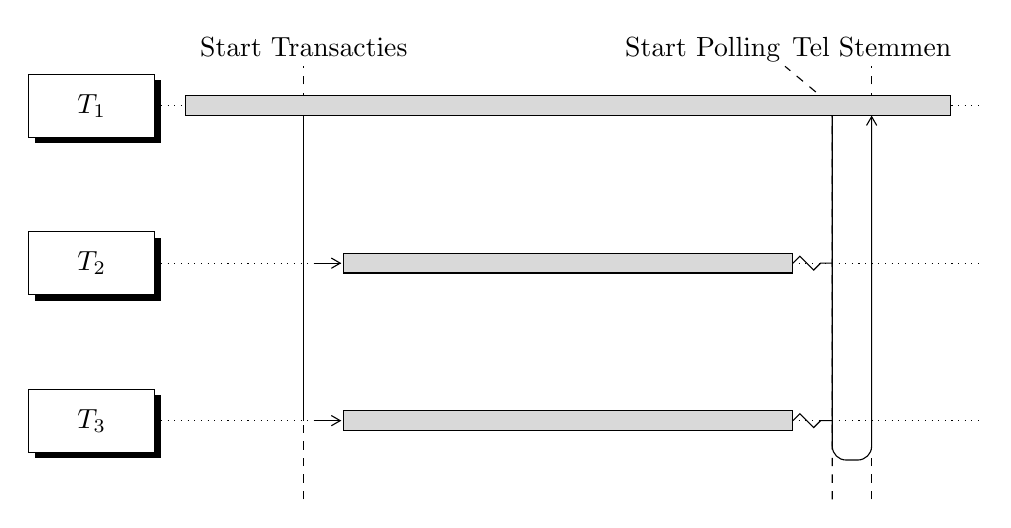
\begin{tikzpicture}
	\setlength{\unitlength}{1cm}
	\tikzstyle{inststyle}=[rectangle, draw, anchor=west, minimum
	height=0.8cm, minimum width=1.6cm, fill=white,
	drop shadow={opacity=1,fill=black}]
\setcounter{threadnum}{1}
\global\def\upperhalfbar{0.125}
\global\def\lowerhalfbar{-\upperhalfbar}
\global\def\twidth{\textwidth-0.4pt}

% tijdlijn met acties
\draw[dashed] (3.5,0) -- (3.5, 5.5) node[above] {Start Transacties};
\draw[dashed] (\twidth-1.9\unitlength,0) -- (\twidth-1.9\unitlength, 5) -- (\twidth-1.9\unitlength,5) --
(\twidth-2.5\unitlength, 5.5) node[above left=-1.79pt] {Start Polling};
\draw[dashed] (\twidth-1.4\unitlength,0) --
(\twidth-1.4\unitlength, 5.5) node[above] {Tel Stemmen};

% Instance 2
\draw[dotted] (0,      \thethreadnum*2-1)
           -- (\twidth,\thethreadnum*2-1)
           node [midway, right=.8\unitlength, below=0.75em] {};
\path (0,0)+(0,1) node[inststyle] (inst1) {\(T_3\)};
\draw[fill=gray!30] (4,\thethreadnum*2-1+\upperhalfbar)
                 -- (4,\thethreadnum*2-1+\lowerhalfbar)
				 -- (\twidth-2.4\unitlength,\thethreadnum*2-1+\lowerhalfbar)
				 --	(\twidth-2.4\unitlength,\thethreadnum*2-1+\upperhalfbar)-- cycle;

\stepcounter{threadnum}

% Instance 2
\draw[dotted] (0,      \thethreadnum*2-1)
           -- (\twidth,\thethreadnum*2-1)
           node [midway, right=.8\unitlength, below=0.75em] {};
\path (0,1)+(0,2) node[inststyle] (inst3) {\(T_2\)};
\draw[fill=gray!30] (4,\thethreadnum*2-1+\upperhalfbar)
                 -- (4,\thethreadnum*2-1+\lowerhalfbar)
				 -- (\twidth-2.4\unitlength,\thethreadnum*2-1+\lowerhalfbar)
				 --	(\twidth-2.4\unitlength,\thethreadnum*2-1+\upperhalfbar)-- cycle;

\stepcounter{threadnum}

% Thread 1
\draw[dotted] (0,      \thethreadnum*2-1)
           -- (\twidth,\thethreadnum*2-1)
           node [midway, right=.8\unitlength, above=0.75em] {};
\path (0,2)+(0,3) node[inststyle] (inst2) {\(T_1\)};
\draw[fill=gray!30] (2,\thethreadnum*2-1+\upperhalfbar)
                 -- (2,\thethreadnum*2-1+\lowerhalfbar)
			     -- (\twidth-.4\unitlength,\thethreadnum*2-1+\lowerhalfbar)
			     -- (\twidth-.4\unitlength,\thethreadnum*2-1+\upperhalfbar)-- cycle;

\stepcounter{threadnum}

% Result/argument arrows
\node (b) at (3.5,5) {};
\node (m) at (3.5,1) {};
\node (e) at (4.1,1) {};
\draw[->,>=angle 60] (b) |- (m) -- (e) node {};

\node (b) at (3.5,5) {};
\node (m) at (3.5,3) {};
\node (e) at (4.1,3) {};
\draw[->,>=angle 60] (b) |- (m) -- (e) node {};

\draw[->,>=angle 60,rounded corners=5pt] (\twidth-1.9\unitlength,5+\lowerhalfbar) %b
                                      -- (\twidth-1.9\unitlength,.5) % m
                                      -- (\twidth-1.4\unitlength,.5) % m'
                                      -- (\twidth-1.4\unitlength,5+\lowerhalfbar); %e

\draw[decorate,decoration=zigzag] {(\twidth-2.4\unitlength, 1) -- (\twidth-1.9\unitlength,1)};
\draw[decorate,decoration=zigzag] {(\twidth-2.4\unitlength, 3) -- (\twidth-1.9\unitlength,3)};

\end{tikzpicture}



\end{document}

